% !TeX root = main.tex

% ============================================================
% thesis-sync entry: 2026-07-19_appendix
% Type: numeric data (raw experimental/FEM tables) + supplementary figures
% Whole-thesis appendix. Must be \input AFTER all normal sections and BEFORE
% the bibliography (\appendix renumbers subsequent sections as A, B, C, ...).
% Requires: graphicx, multirow, makecell.
% Data sources: figures/appendix_figures/{ComsolResults.xlsx, 3x Actuator.xlsx}.
% ============================================================

\appendix

\section{FEM Simulation Data}
\label{app:fem-data}

Tables~\ref{tab:app-wallthickness}--\ref{tab:app-designcomparison} report the
tabulated bending angles obtained from the COMSOL finite-element studies of
the omnidirectional actuator (Section~\ref{sec:inchworm-actuator}).

\begin{table}[tbh]
  \caption{Wall-thickness study: bending angle versus silicone outer-wall
  thickness, single chamber pressurized at 3~kPa.}
  \label{tab:app-wallthickness}
  \centering
  \footnotesize
  \begin{tabular}{|c|c|}
    \hline
    Wall thickness [mm] & Bending angle [deg] \\ \hline
    0.2 & 37.09 \\ \hline
    0.3 & 13.14 \\ \hline
    0.4 & 6.62 \\ \hline
    0.5 & 4.46 \\ \hline
  \end{tabular}
\end{table}

\begin{table}[tbh]
  \caption{Fiber-spacing study: bending angle versus circumferential fiber
  spacing, single chamber pressurized at 2~kPa.}
  \label{tab:app-fiberspacing}
  \centering
  \footnotesize
  \begin{tabular}{|c|c|}
    \hline
    Fiber spacing [mm] & Bending angle [deg] \\ \hline
    1 & 20.58 \\ \hline
    2 & 16.23 \\ \hline
    3 & 13.23 \\ \hline
    4 & 11.34 \\ \hline
    5 & 10.70 \\ \hline
  \end{tabular}
\end{table}

\begin{table}[tbh]
  \caption{Design-comparison study: bending angle for one and two
  simultaneously pressurized chambers at 3~kPa (3~mm circumferential fiber
  spacing) across the three candidate designs.}
  \label{tab:app-designcomparison}
  \centering
  \footnotesize
  \setlength{\tabcolsep}{5pt}
  \begin{tabular}{|l|c|c|}
    \hline
    Design & \makecell{1 chamber\\{[}deg{]}} & \makecell{2 chambers\\{[}deg{]}} \\ \hline
    Baseline (EcoFlex 00-30) & 37.09 & 28.74 \\ \hline
    Dual-material (EcoFlex 00-50 walls) & 27.81 & 24.69 \\ \hline
    Radial fibers (3~mm) & 20.13 & 26.06 \\ \hline
  \end{tabular}
\end{table}

\section{Actuator Characterization Data}
\label{app:actuator-data}

Tables~\ref{tab:app-fullscale}--\ref{tab:app-mini-fiber} report the raw
single-chamber pressure--angle measurements behind the bending
characterization of Section~\ref{sec:inchworm-bending-experiment} and of the
miniaturization study of Section~\ref{sec:lizard-characterization}. The
displacements $x$ and $y$ denote the horizontal and vertical coordinates of
the actuator tip relative to its rest position.

\begin{table}[tbh]
  \caption{Full-scale segment ($L=60$~mm bendable length), single chamber,
  measured over a full inflation (top) and deflation (bottom) cycle.}
  \label{tab:app-fullscale}
  \centering
  \footnotesize
  \setlength{\tabcolsep}{5pt}
  \begin{tabular}{|c|c|c|c|}
    \hline
    \makecell{Pressure\\{[}kPa{]}} & \makecell{Bending\\angle [deg]} & \makecell{Displ. $x$\\{[}mm{]}} & \makecell{Displ. $y$\\{[}mm{]}} \\ \hline
    0.0 & 0.0 & 0.0 & 0.0 \\ \hline
    1.2 & 7.4 & 2.6 & -1.0 \\ \hline
    2.2 & 11.8 & 5.4 & -1.3 \\ \hline
    3.1 & 13.2 & 6.6 & -1.3 \\ \hline
    4.3 & 19.7 & 10.9 & -1.4 \\ \hline
    5.4 & 28.3 & 14.8 & -1.0 \\ \hline
    6.2 & 35.6 & 19.3 & -0.1 \\ \hline
    7.2 & 43.3 & 25.9 & 1.5 \\ \hline
    8.1 & 54.3 & 33.4 & 4.7 \\ \hline
    9.2 & 71.7 & 42.8 & 9.9 \\ \hline
    10.2 & 93.2 & 49.7 & 17.2 \\ \hline
    11.2 & 120.6 & 54.9 & 27.1 \\ \hline
    12.2 & 135.5 & 58.3 & 38.6 \\ \hline
    13.2 & 155.3 & 59.3 & 47.8 \\ \hline
    14.2 & 170.0 & 57.4 & 56.1 \\ \hline
    14.8 & 181.4 & 55.4 & 61.9 \\ \hline
    14.6 & 174.9 & 56.7 & 57.6 \\ \hline
    13.0 & 158.2 & 58.4 & 48.6 \\ \hline
    12.2 & 141.2 & 58.1 & 40.1 \\ \hline
    11.2 & 126.2 & 56.5 & 31.9 \\ \hline
    10.3 & 102.4 & 51.7 & 20.9 \\ \hline
    9.1 & 87.2 & 45.9 & 13.4 \\ \hline
    7.2 & 56.3 & 31.7 & 3.6 \\ \hline
    6.1 & 30.5 & 18.3 & 0.6 \\ \hline
    5.0 & 24.6 & 13.7 & -1.3 \\ \hline
    4.1 & 18.4 & 10.9 & -1.8 \\ \hline
    3.3 & 13.3 & 7.0 & -1.5 \\ \hline
    2.1 & 9.5 & 4.4 & -1.2 \\ \hline
    1.0 & 3.1 & 1.7 & -0.6 \\ \hline
    0.0 & 0.0 & 0.0 & 0.0 \\ \hline
  \end{tabular}
\end{table}

\begin{table}[tbh]
  \caption{Miniaturized segment ($L=20$~mm bendable length) without the
  central axial fiber, single chamber, during inflation.}
  \label{tab:app-mini-nofiber}
  \centering
  \footnotesize
  \setlength{\tabcolsep}{5pt}
  \begin{tabular}{|c|c|c|c|}
    \hline
    \makecell{Pressure\\{[}kPa{]}} & \makecell{Bending\\angle [deg]} & \makecell{Displ. $x$\\{[}mm{]}} & \makecell{Displ. $y$\\{[}mm{]}} \\ \hline
    0.0 & 0.0 & 0.0 & 0.0 \\ \hline
    1.1 & 4.7 & 1.1 & -0.2 \\ \hline
    3.1 & 10.9 & 3.1 & -0.6 \\ \hline
    4.3 & 14.7 & 4.2 & -0.5 \\ \hline
    5.4 & 22.3 & 6.2 & -0.4 \\ \hline
    7.5 & 28.5 & 9.0 & 0.1 \\ \hline
    8.9 & 38.9 & 11.8 & 1.3 \\ \hline
    9.9 & 54.0 & 16.4 & 3.2 \\ \hline
    10.8 & 60.3 & 17.9 & 3.8 \\ \hline
    11.7 & 71.0 & 20.1 & 5.3 \\ \hline
    13.0 & 99.2 & 25.6 & 12.1 \\ \hline
    14.0 & 121.7 & 27.9 & 18.2 \\ \hline
    15.5 & 152.0 & 27.9 & 27.4 \\ \hline
    16.4 & 172.6 & 25.6 & 32.4 \\ \hline
  \end{tabular}
\end{table}

\begin{table}[tbh]
  \caption{Miniaturized segment ($L=20$~mm bendable length) with the central
  axial fiber, single chamber, during inflation.}
  \label{tab:app-mini-fiber}
  \centering
  \footnotesize
  \setlength{\tabcolsep}{6pt}
  \begin{tabular}{|c|c|}
    \hline
    Pressure [kPa] & Bending angle [deg] \\ \hline
    0.1 & 0.0 \\ \hline
    2.5 & 6.1 \\ \hline
    3.9 & 11.3 \\ \hline
    5.3 & 15.6 \\ \hline
    6.6 & 17.7 \\ \hline
    7.7 & 30.5 \\ \hline
    8.8 & 39.1 \\ \hline
    9.5 & 52.3 \\ \hline
    10.6 & 65.9 \\ \hline
    11.2 & 77.6 \\ \hline
    11.9 & 86.4 \\ \hline
    12.7 & 105.9 \\ \hline
    13.4 & 124.1 \\ \hline
    13.8 & 138.6 \\ \hline
    14.2 & 148.9 \\ \hline
    14.5 & 158.3 \\ \hline
    15.0 & 178.8 \\ \hline
  \end{tabular}
\end{table}

\section{Supplementary Figures}
\label{app:figures}

\begin{figure}[tbh]
  \centering
  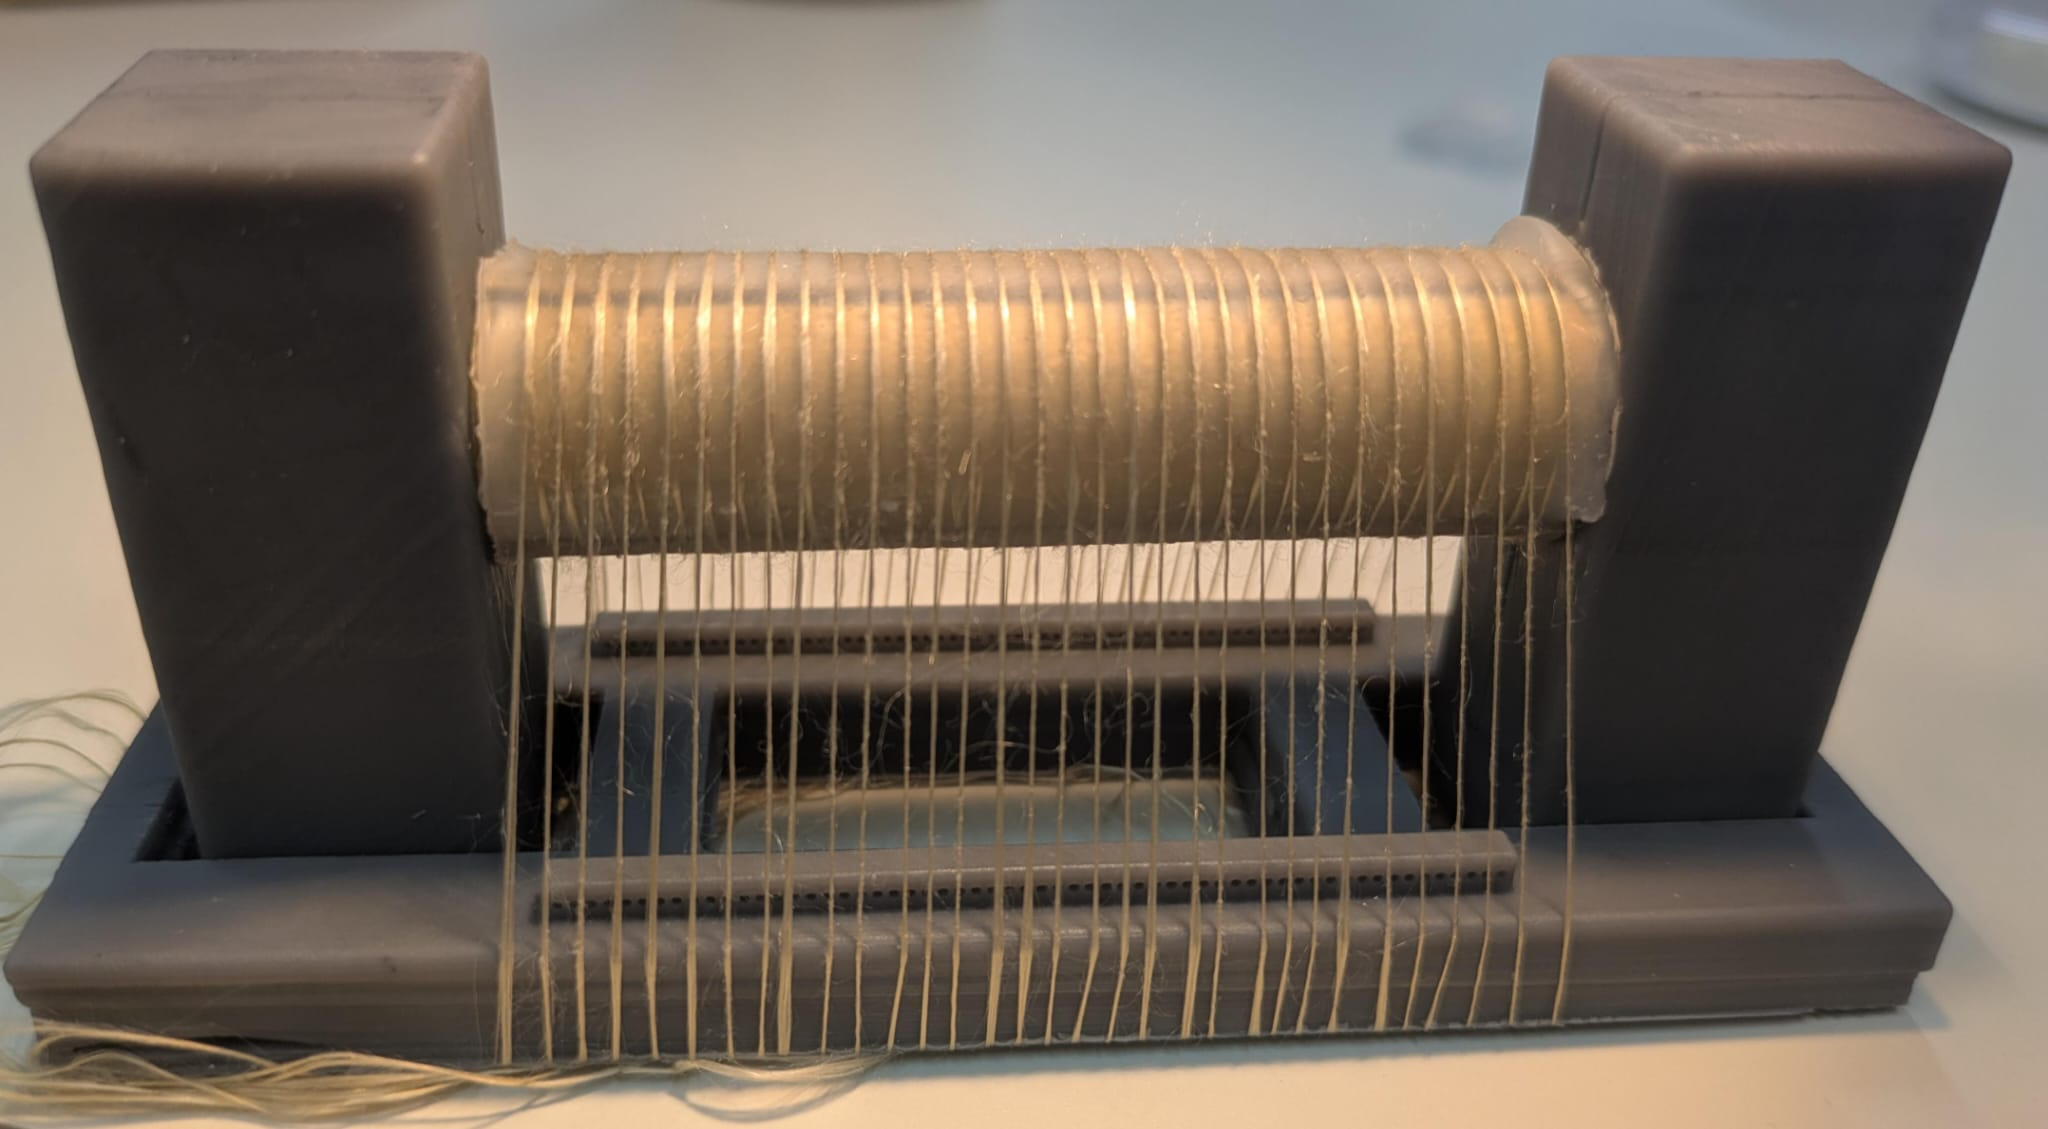
\includegraphics[width=0.85\columnwidth]{figures/appendix_figures/fibers3x.jpeg}
  \vspace*{-1mm}
  \caption{Circumferential fiber reinforcement wound around the silicone
  actuator body during fabrication (Section~\ref{sec:inchworm-fabrication}).}
  \label{fig:app-fibers}
\end{figure}

\begin{figure}[tbh]
  \centering
  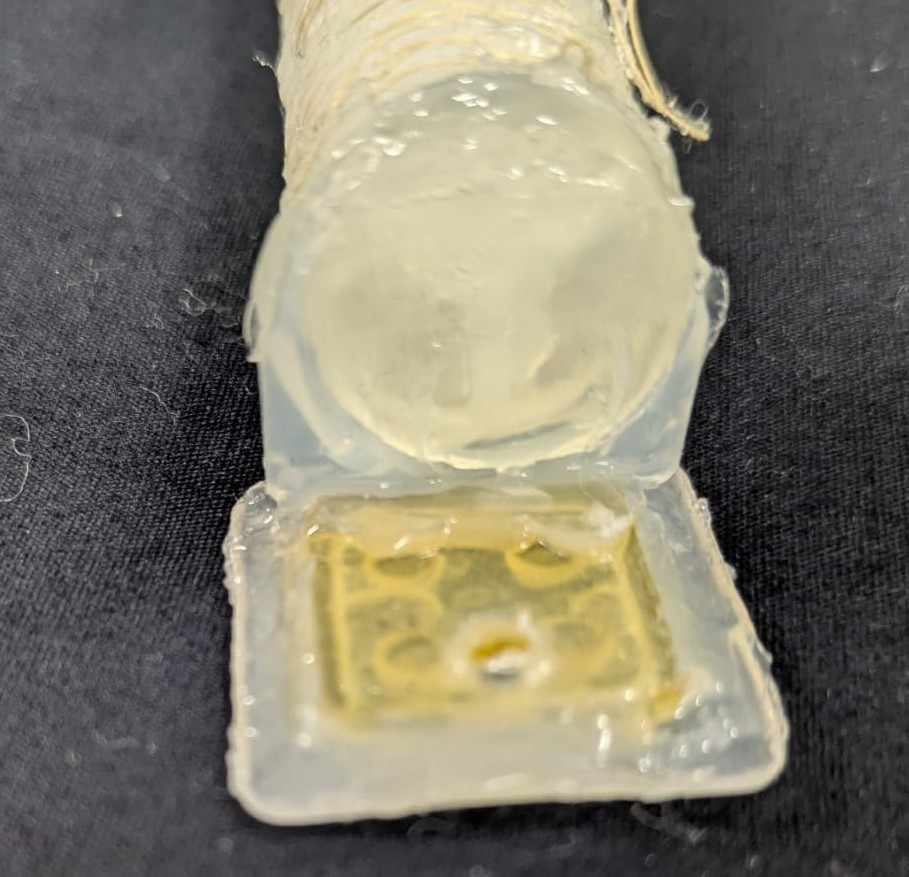
\includegraphics[height=34mm]{figures/appendix_figures/softHinge.jpeg}
  \hspace{3mm}
  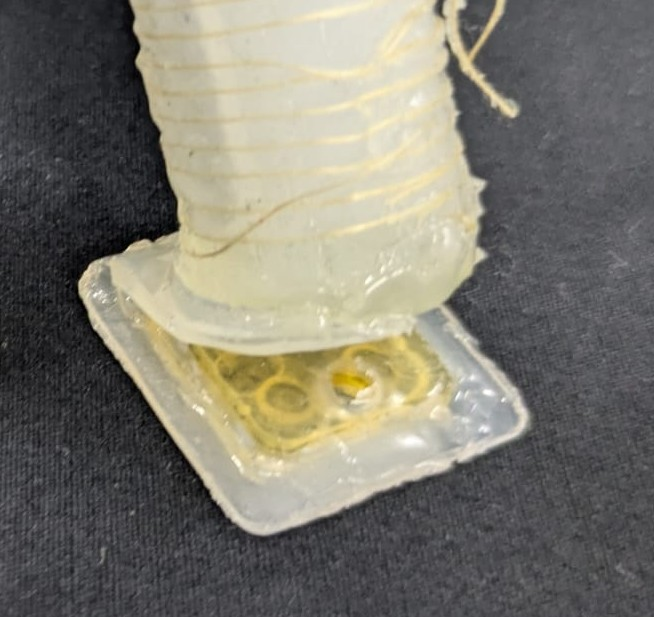
\includegraphics[height=34mm]{figures/appendix_figures/softHingebent.jpeg}
  \vspace*{-1mm}
  \caption{Soft passive hinge bonding a suction-cup foot to the actuator
  extremity. (Left) At rest, the foot is coaxial with the actuator. (Right)
  The compliant hinge lets the foot passively rotate to stay flat on the
  surface while the actuator bends.}
  \label{fig:app-hinge}
\end{figure}

\begin{figure*}[tbh]
  \centering
  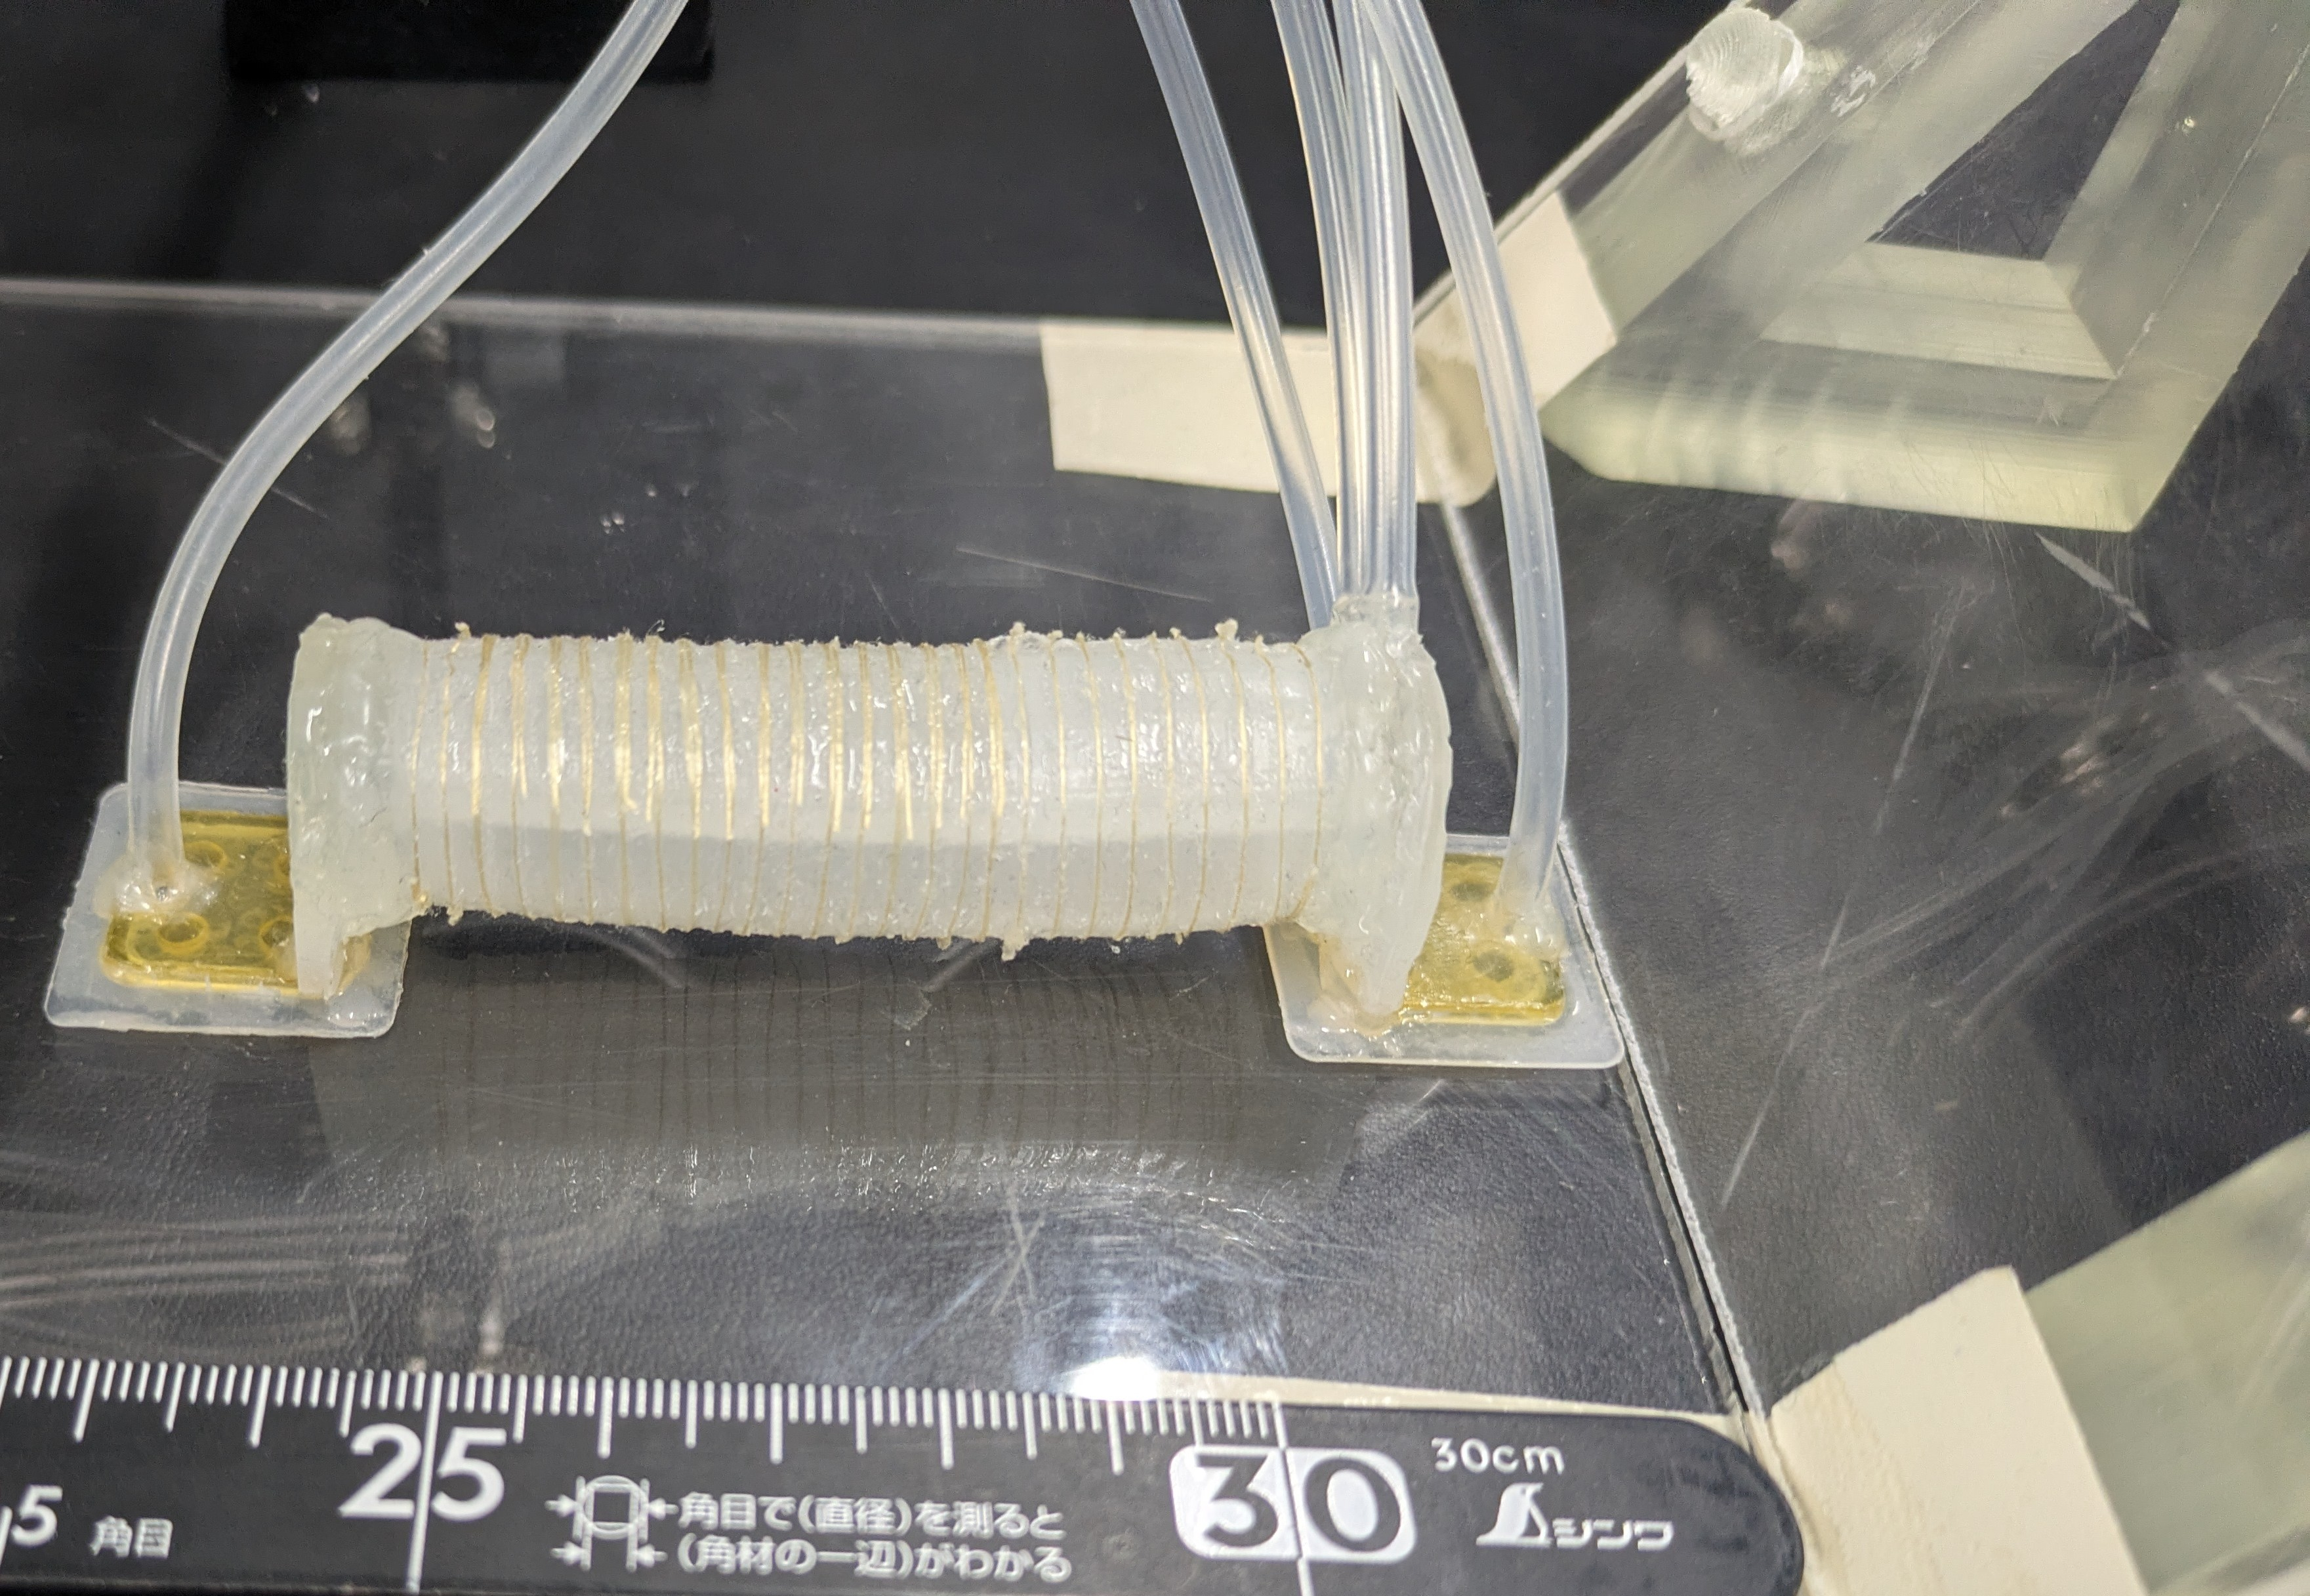
\includegraphics[width=0.185\textwidth]{figures/appendix_figures/1.jpg}\hfill
  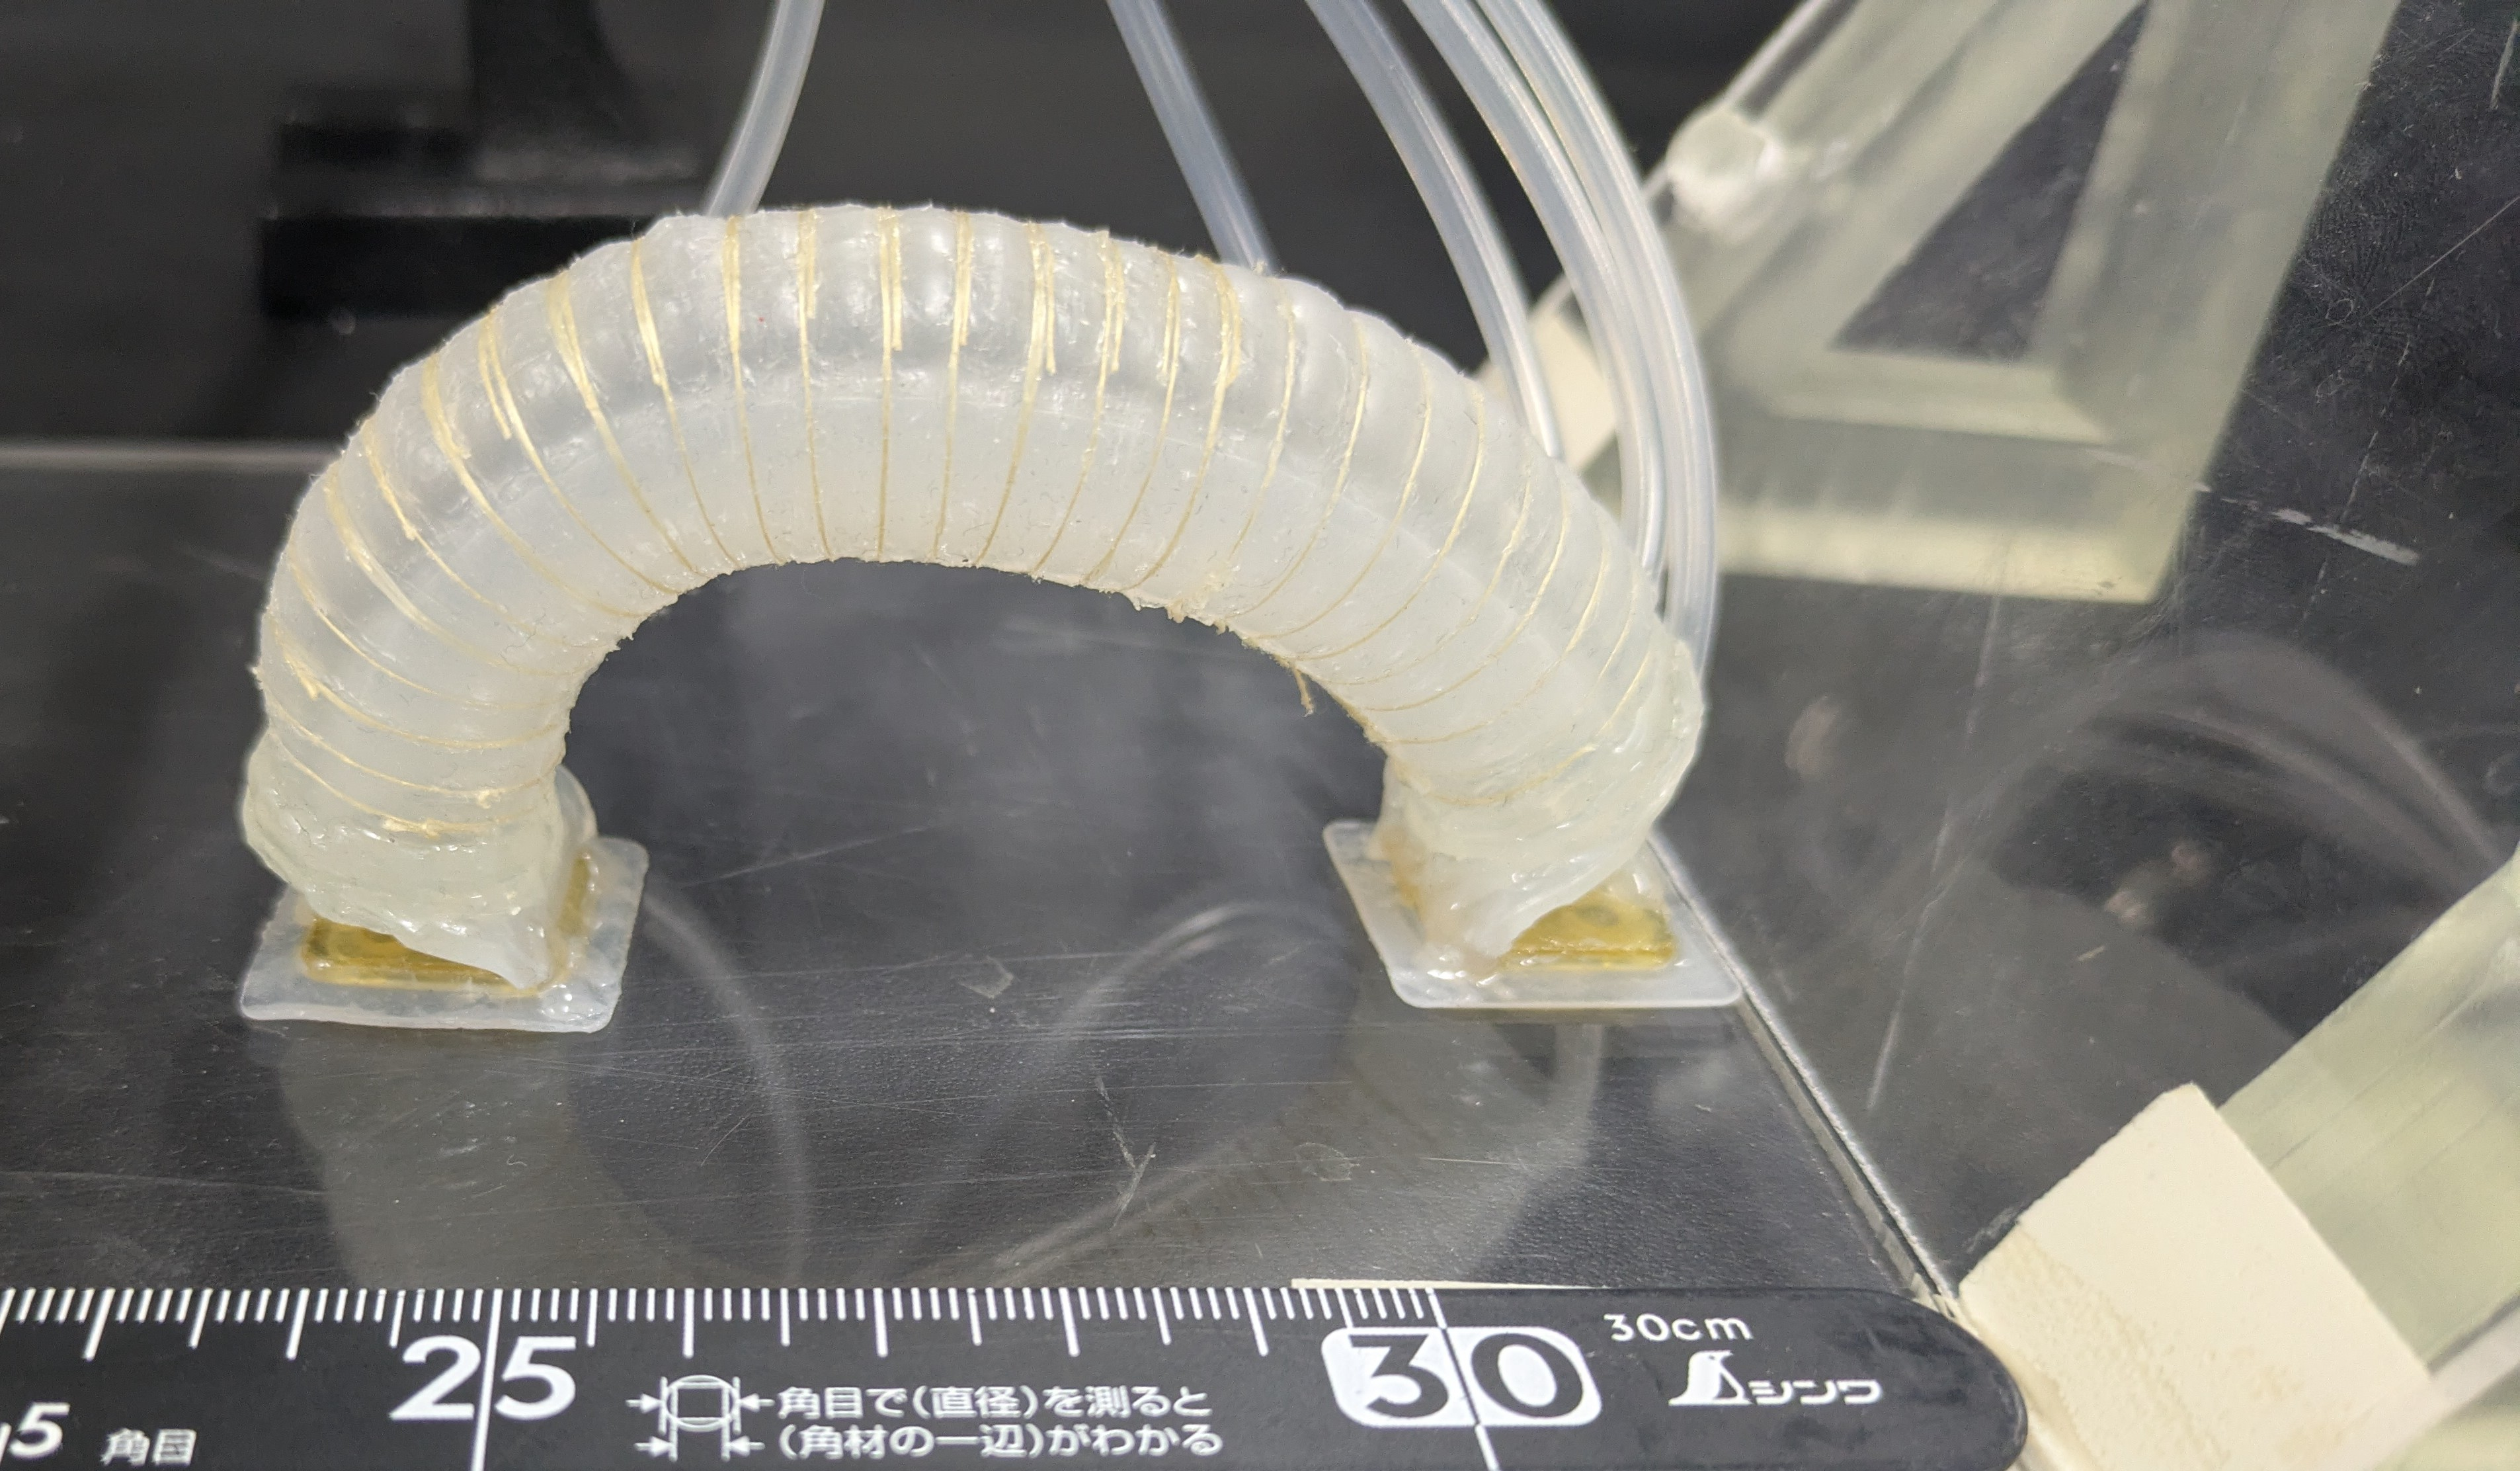
\includegraphics[width=0.185\textwidth]{figures/appendix_figures/2.jpg}\hfill
  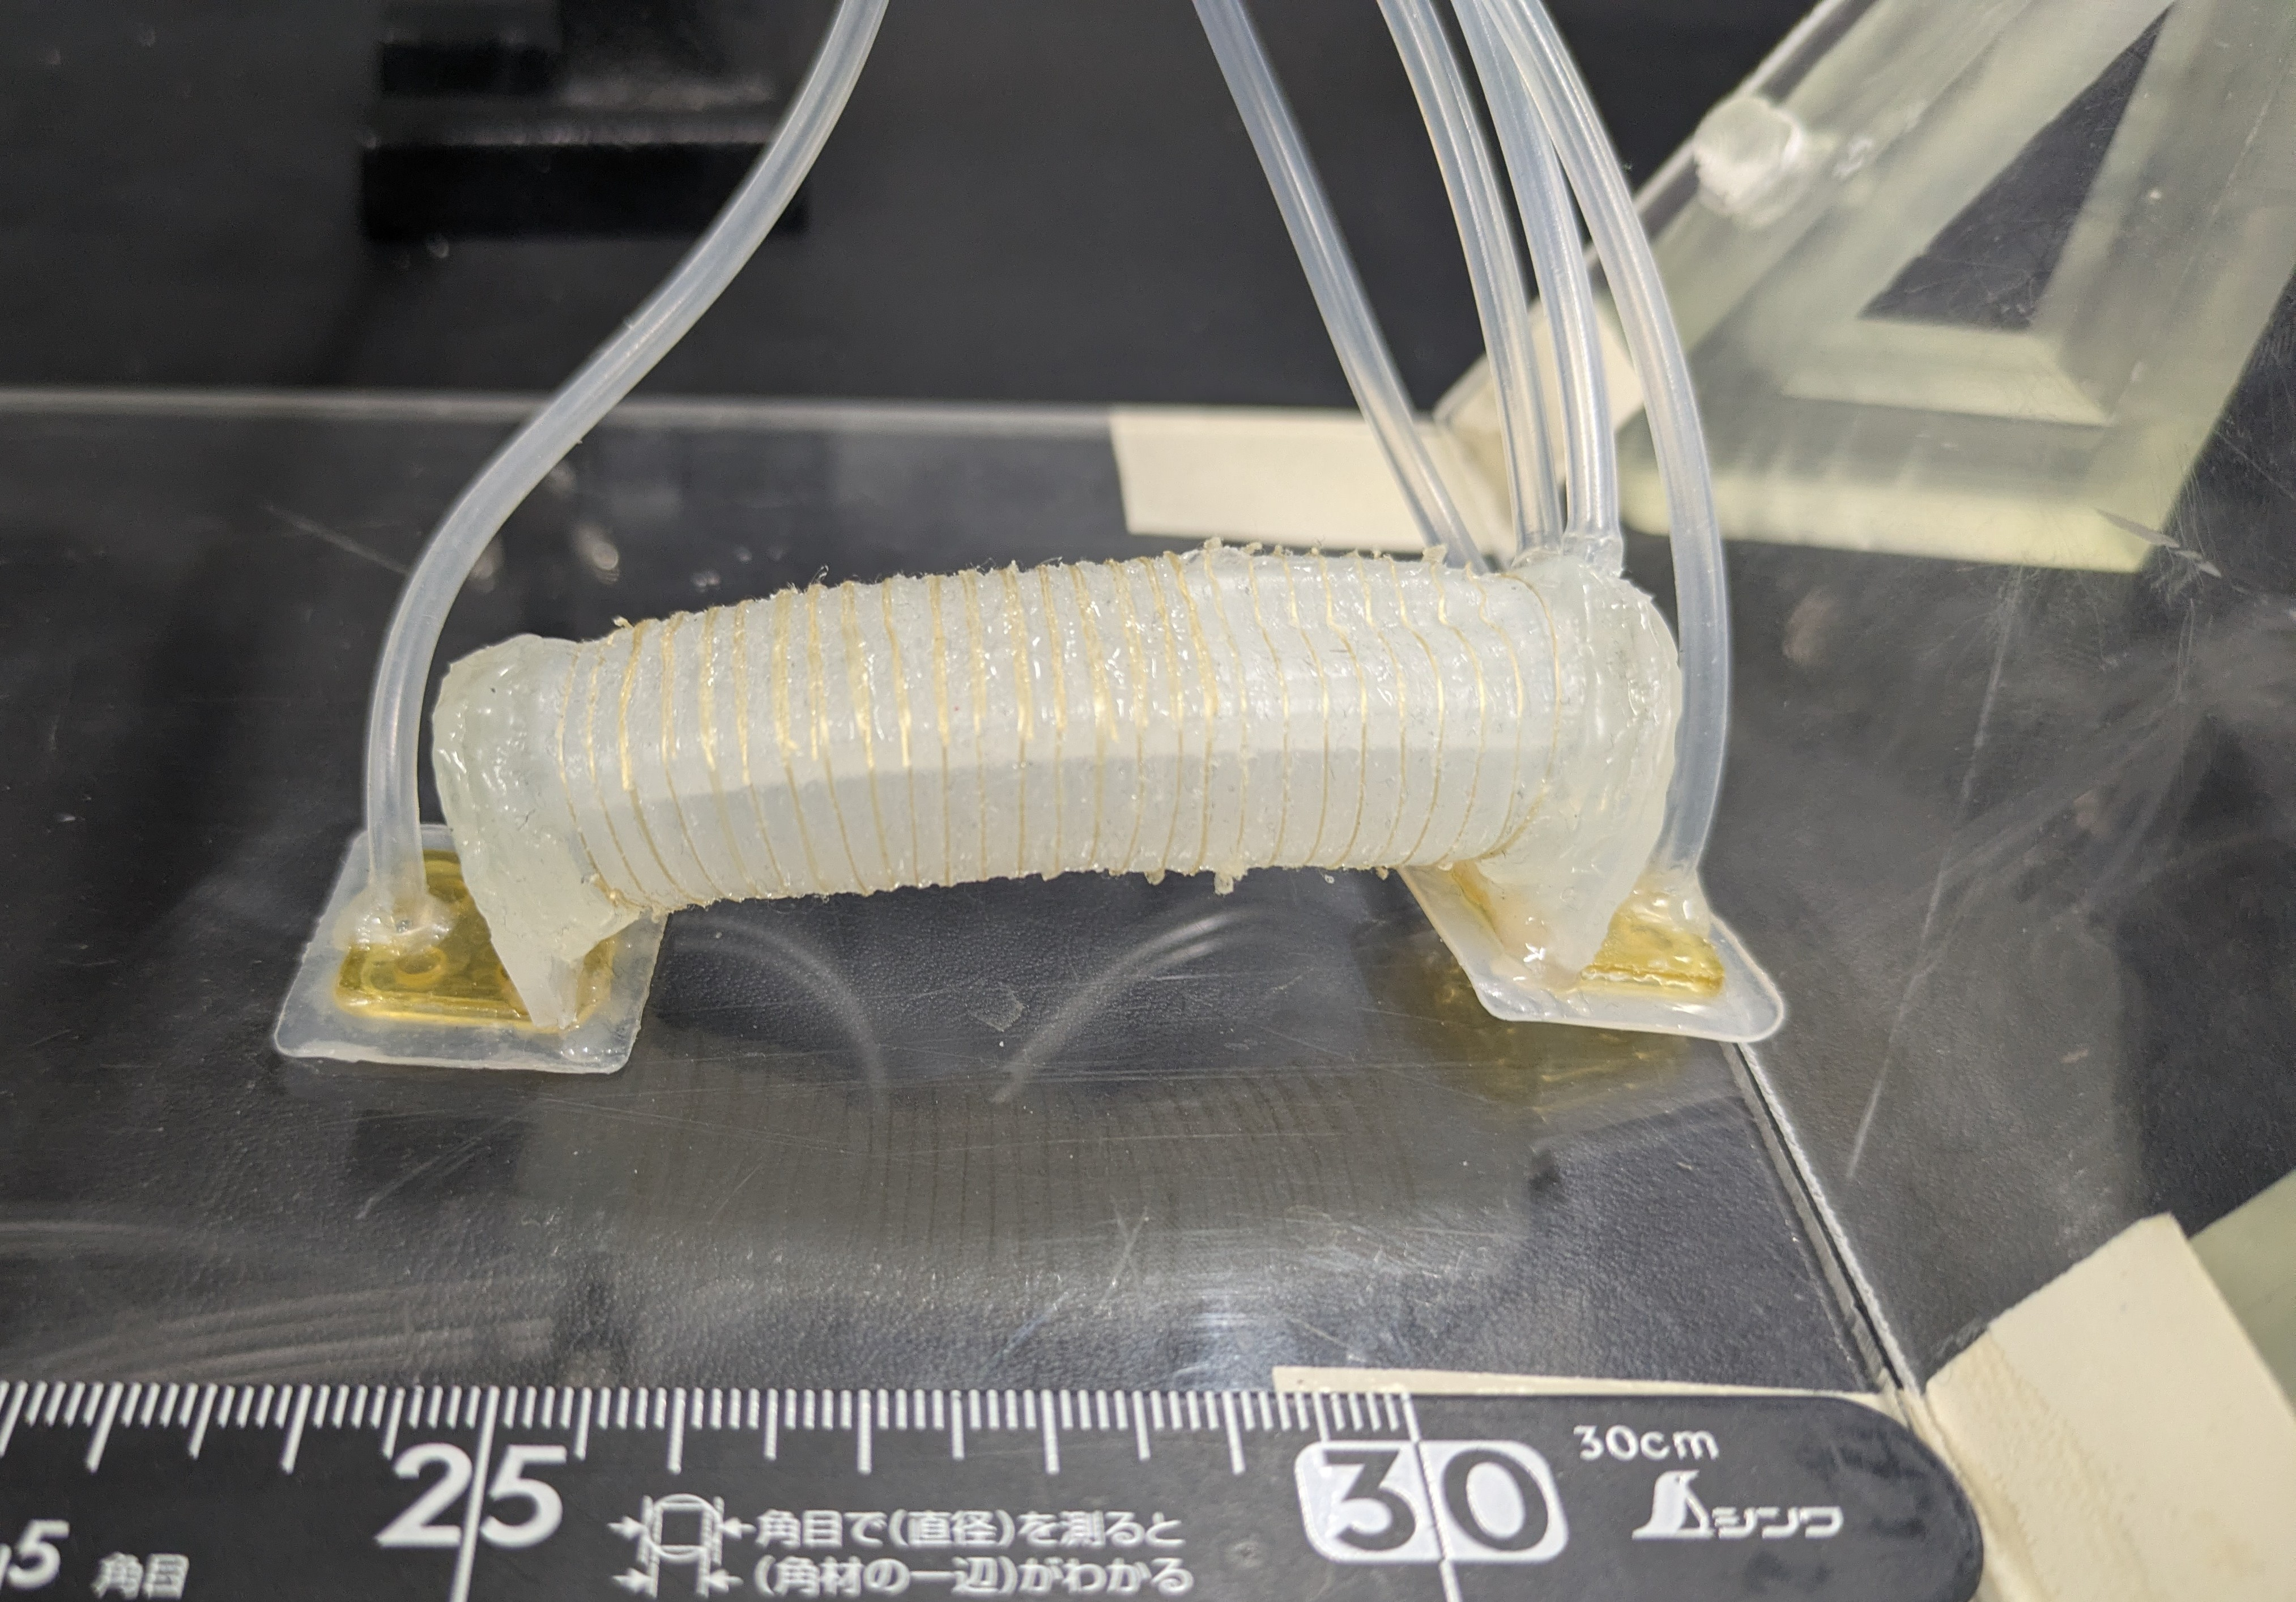
\includegraphics[width=0.185\textwidth]{figures/appendix_figures/3.jpg}\hfill
  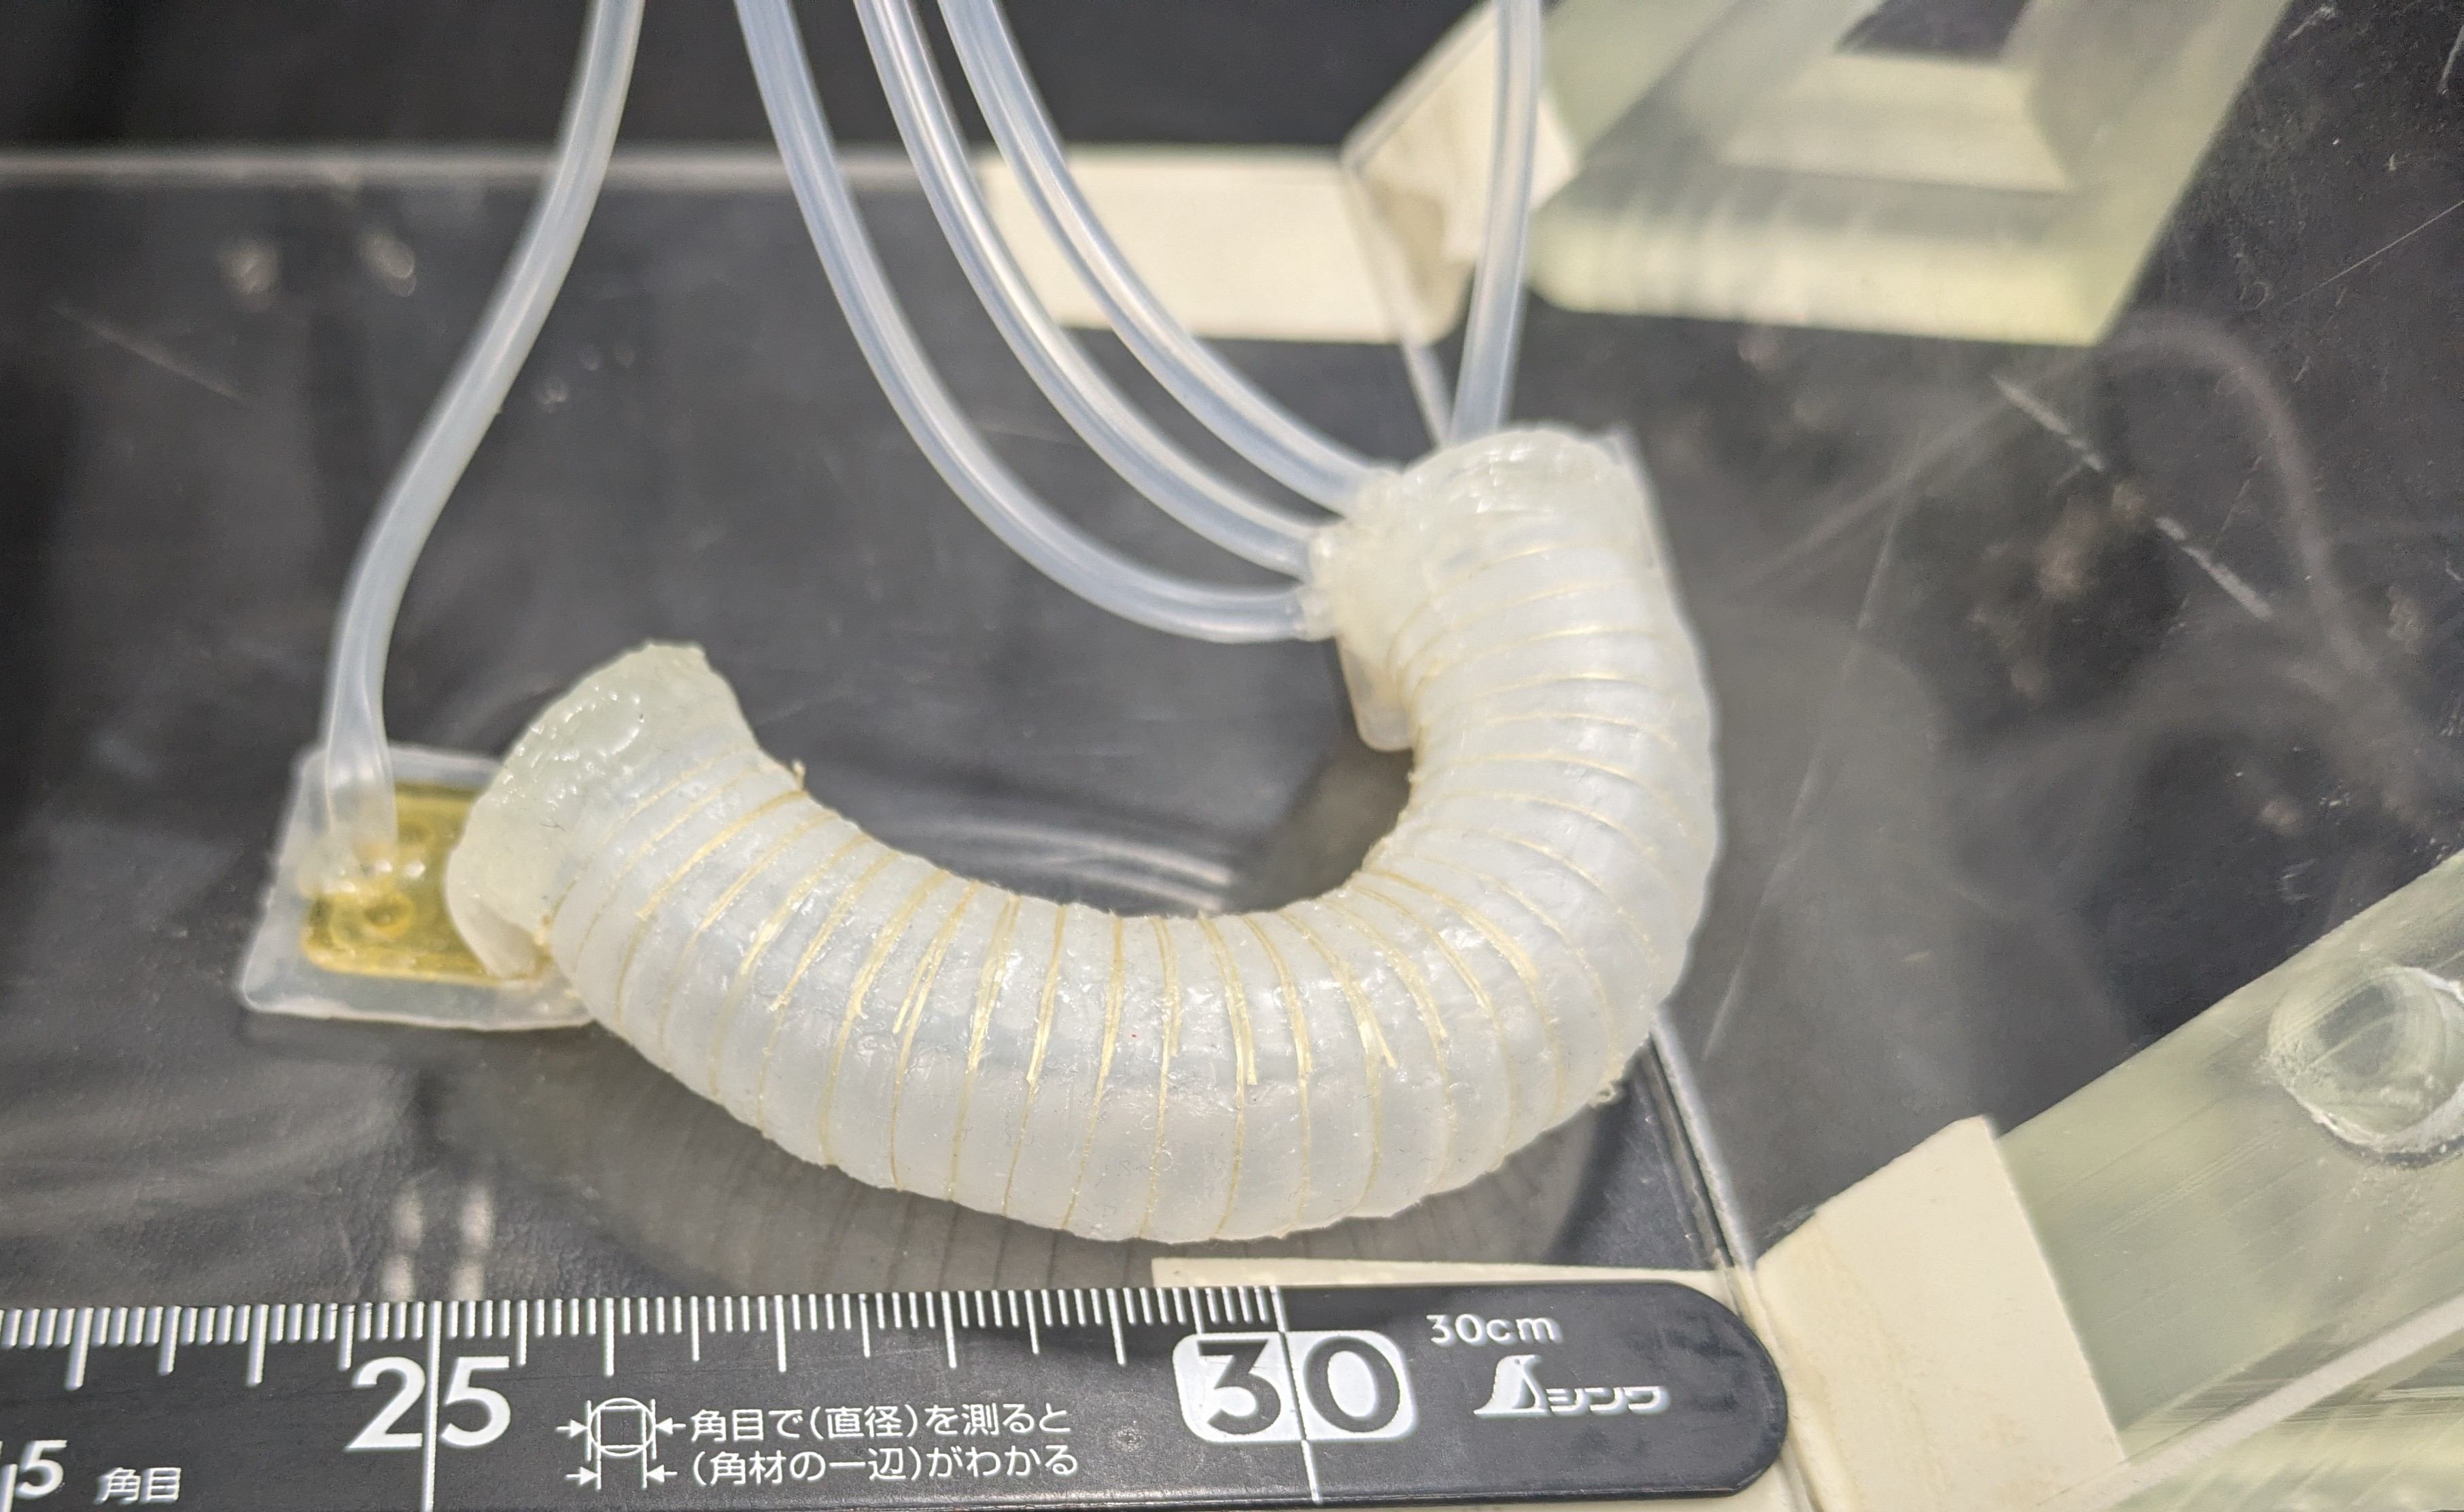
\includegraphics[width=0.185\textwidth]{figures/appendix_figures/4.jpg}\hfill
  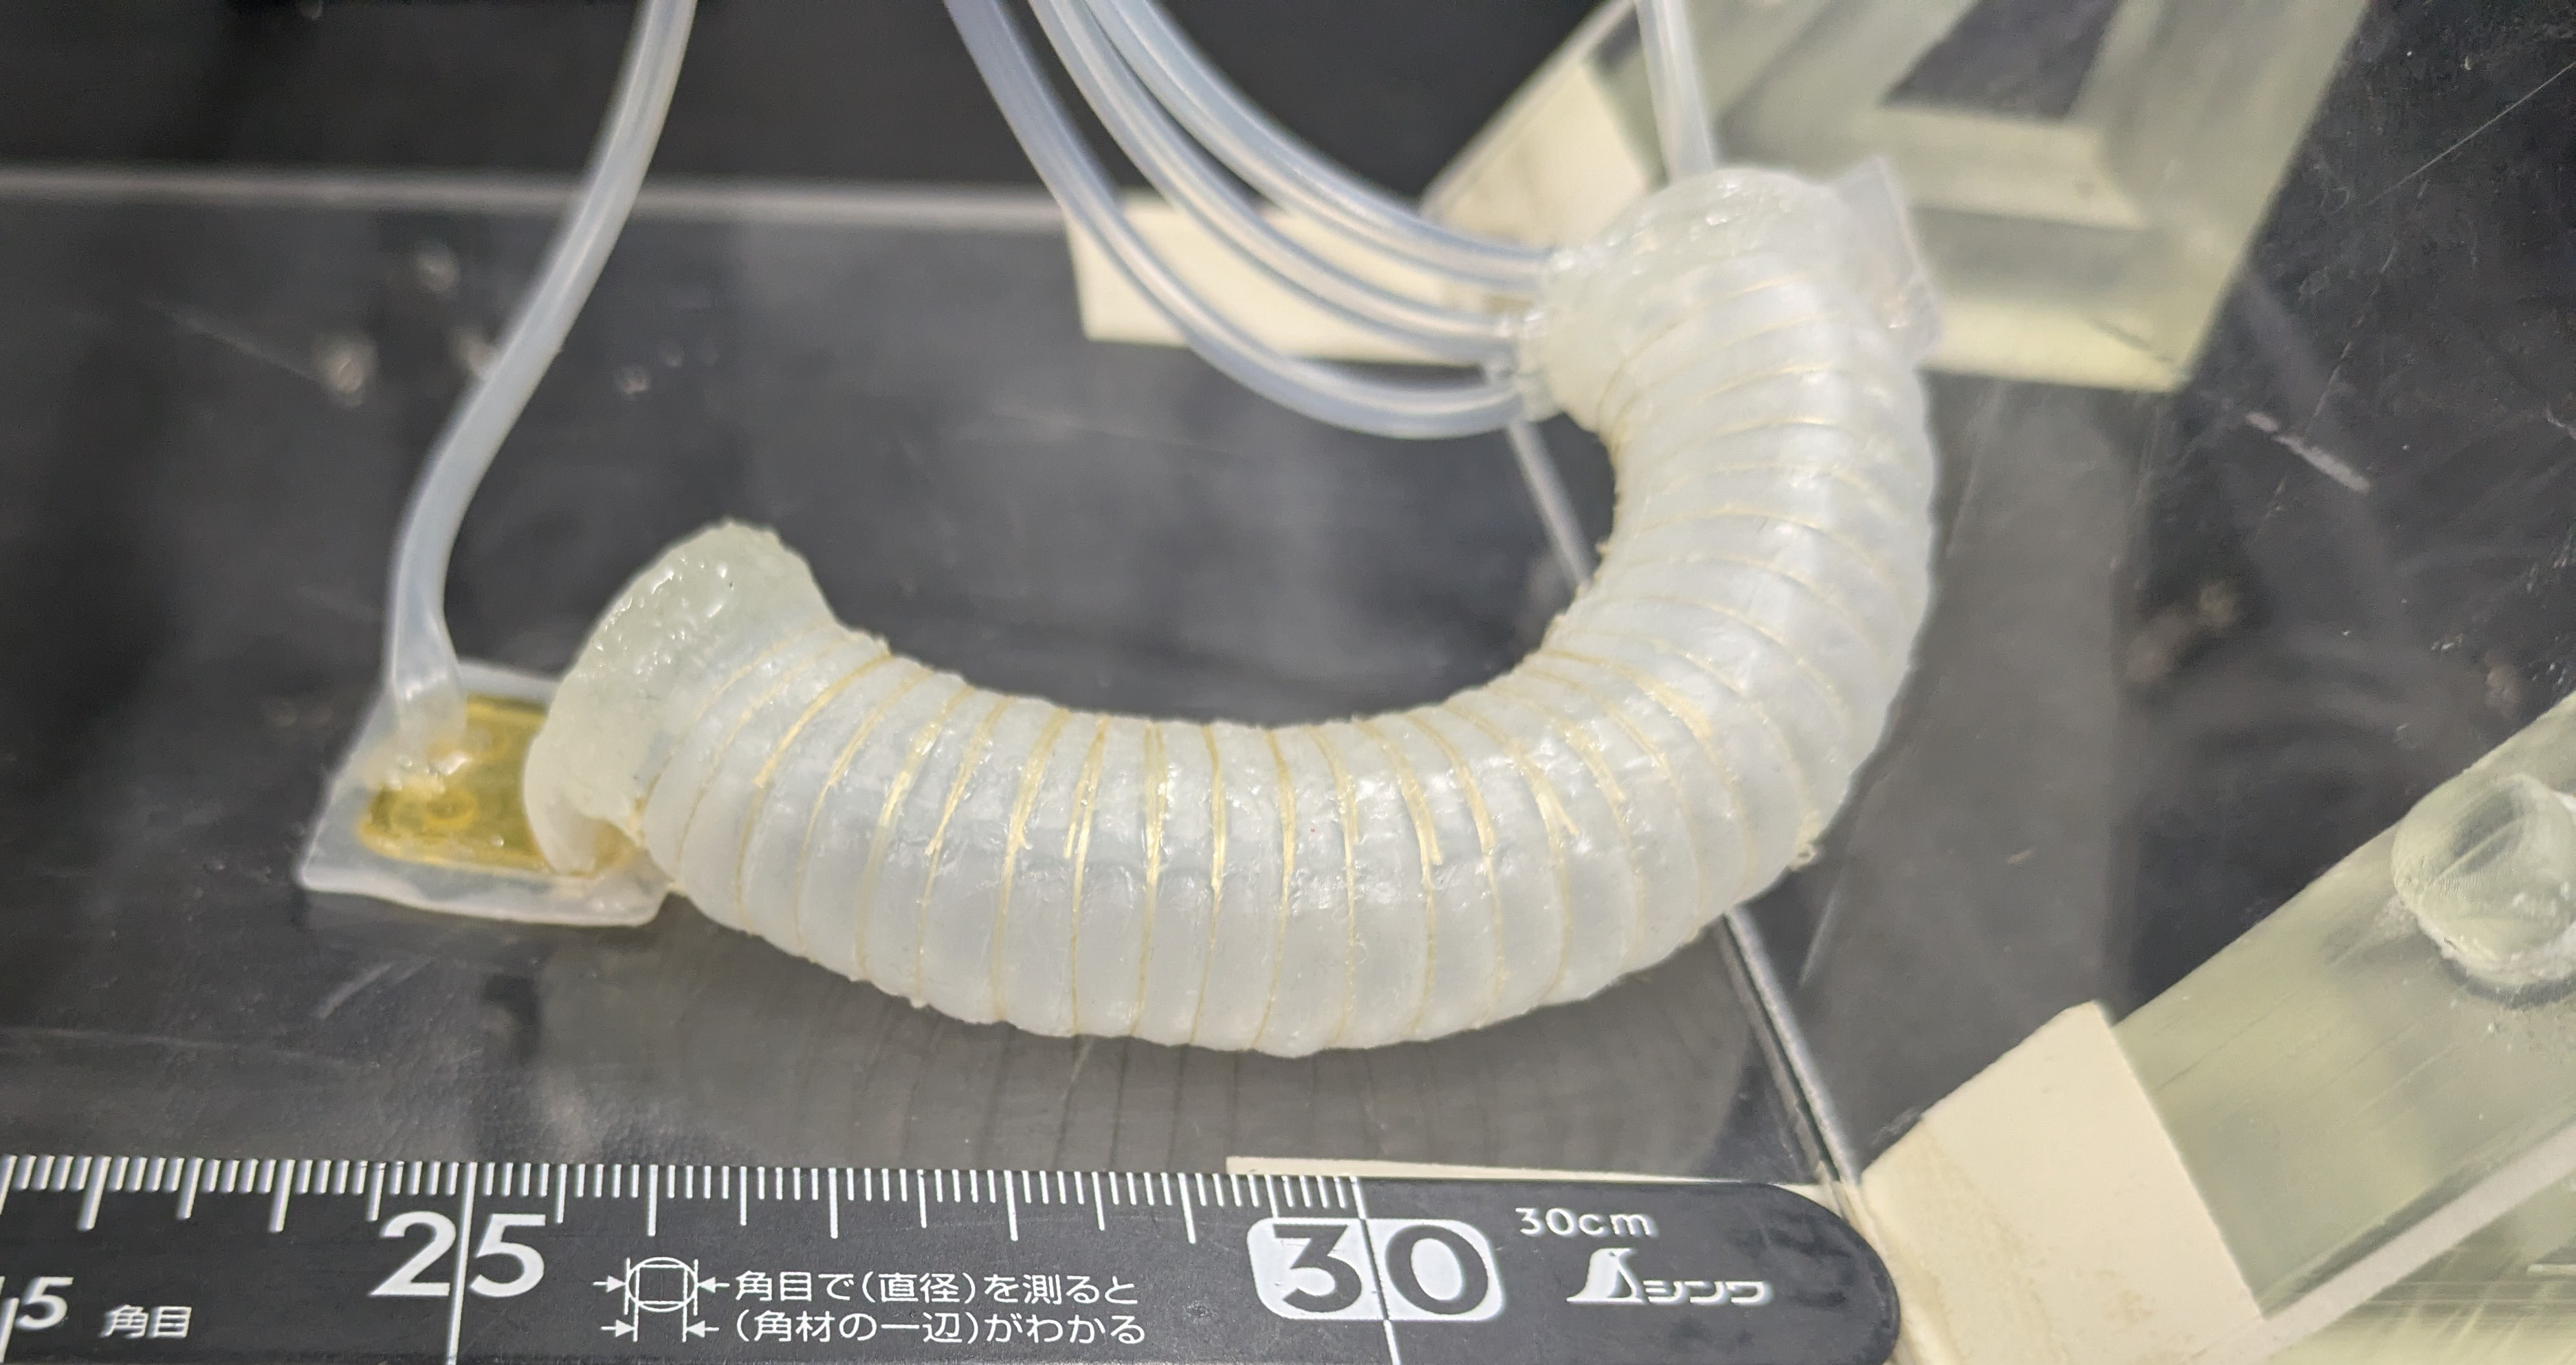
\includegraphics[width=0.185\textwidth]{figures/appendix_figures/5.jpg}
  \\[1.5mm]
  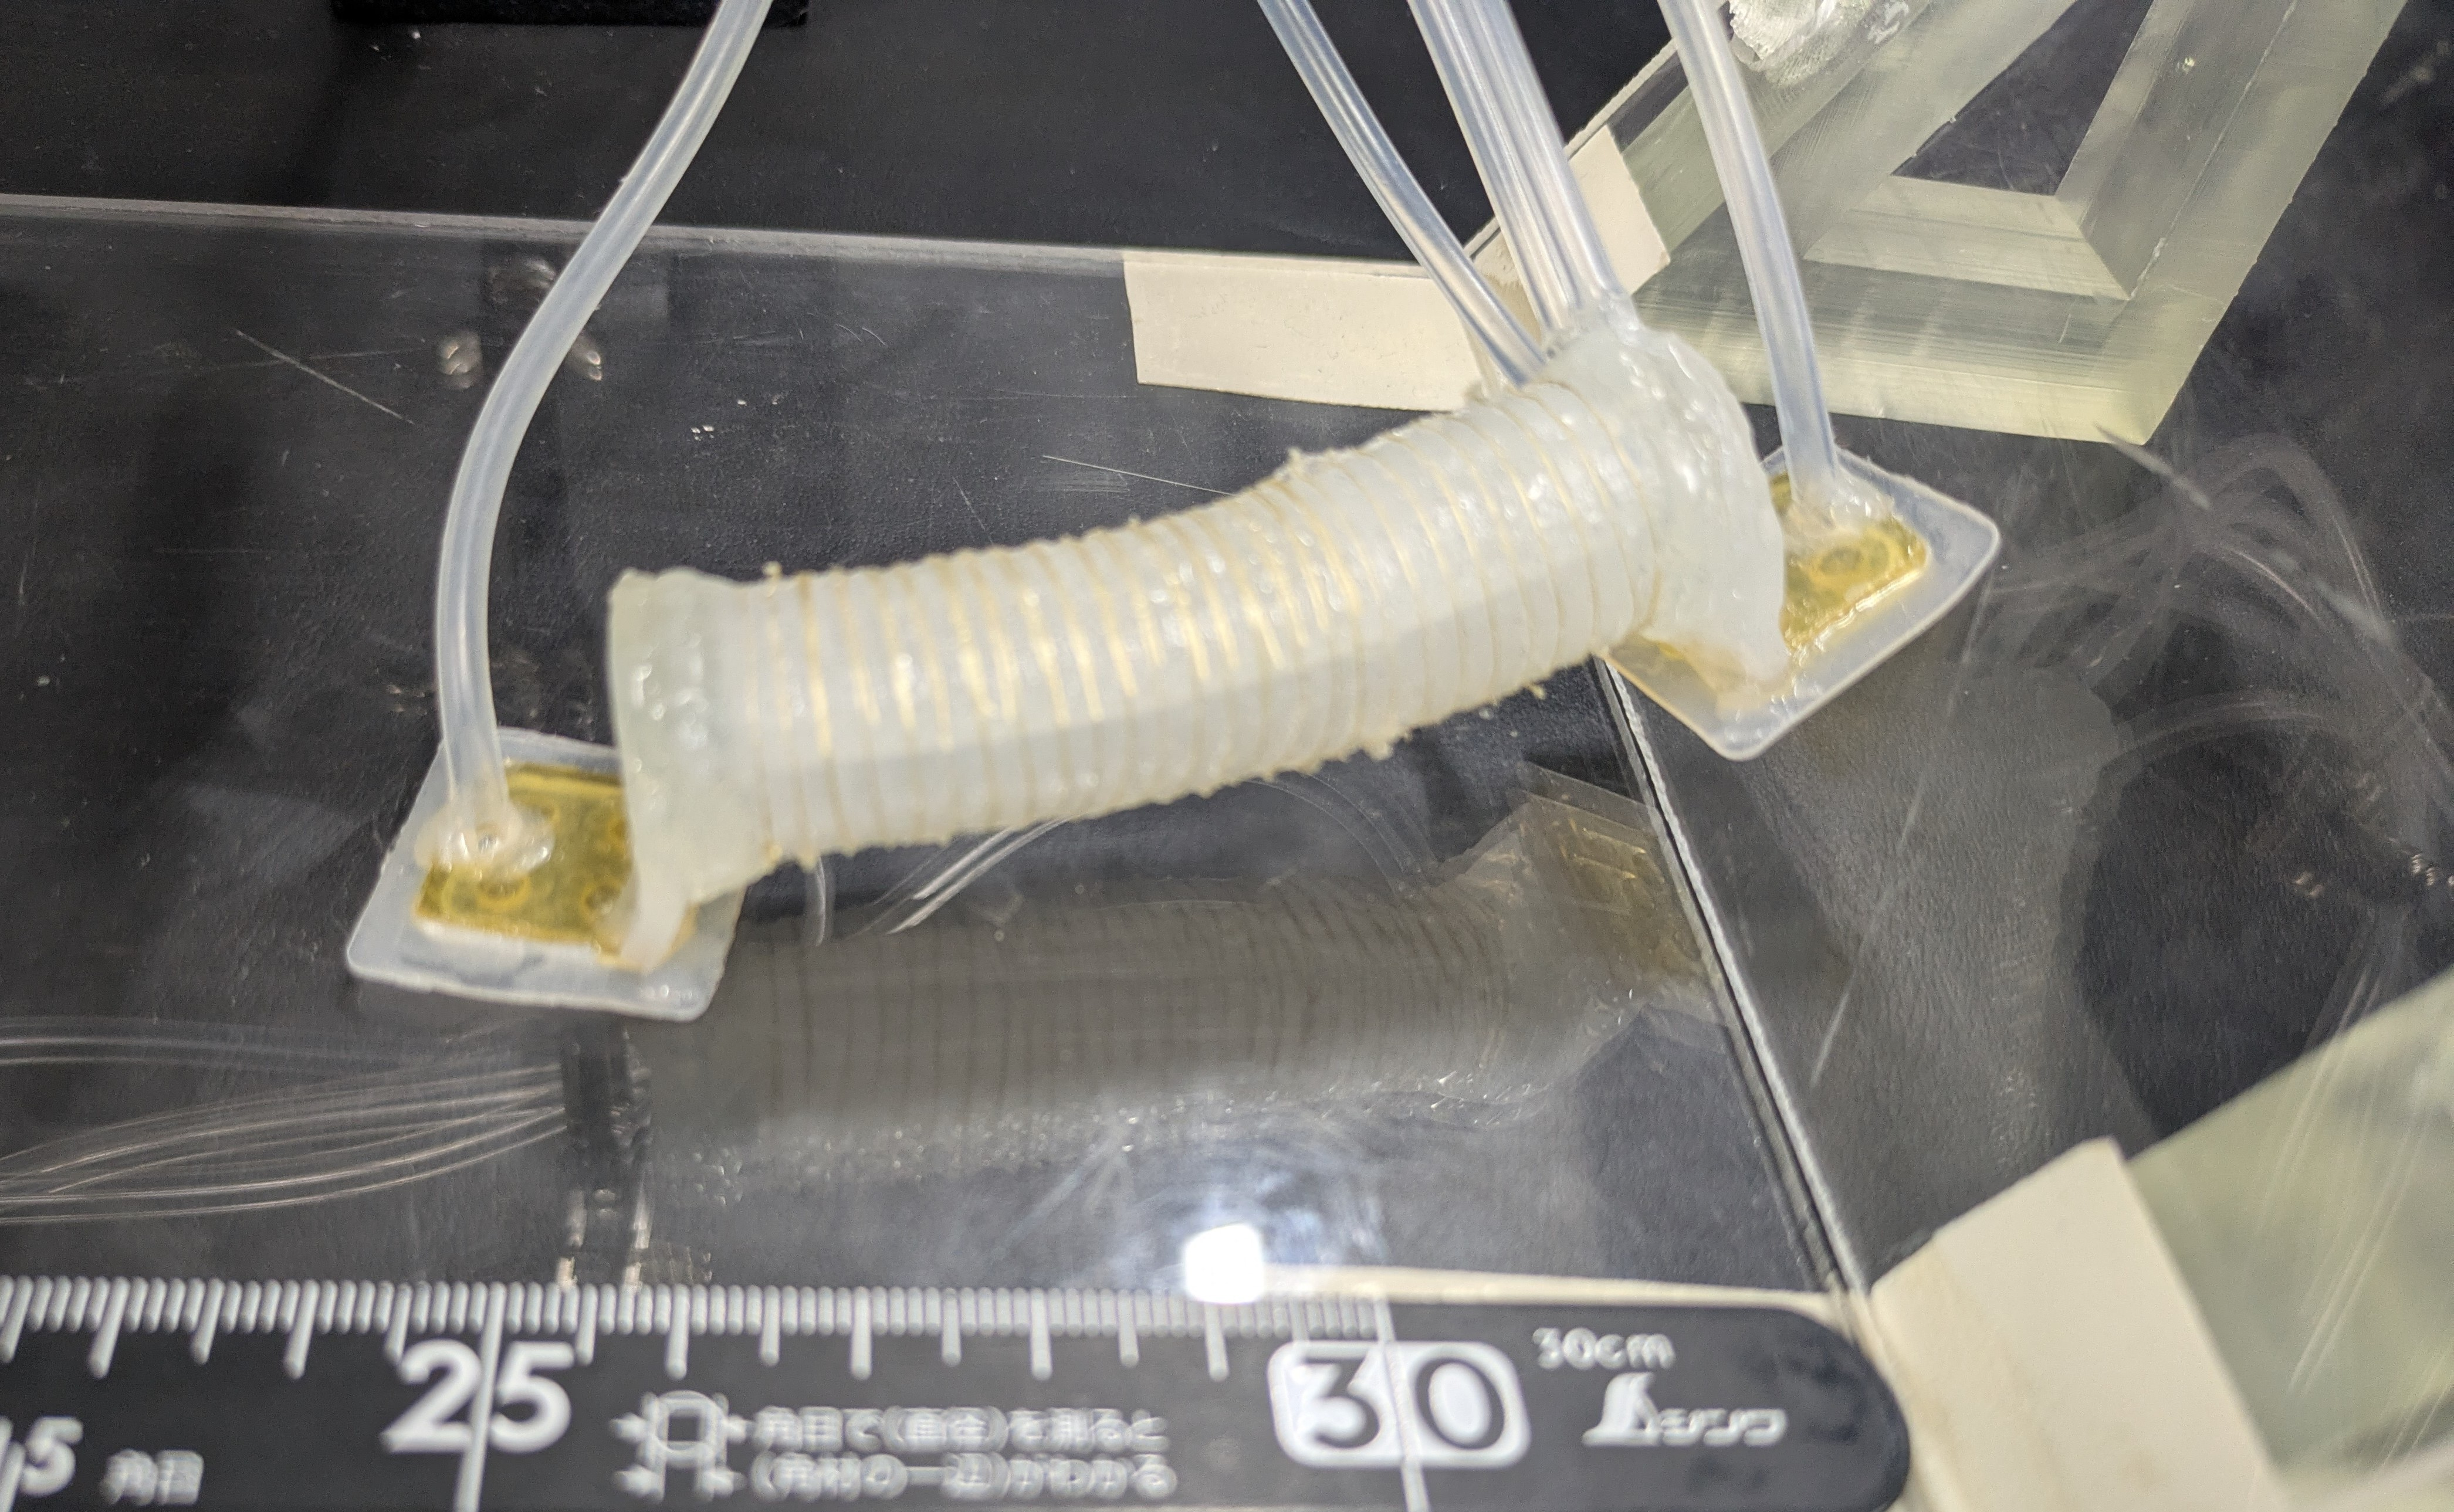
\includegraphics[width=0.185\textwidth]{figures/appendix_figures/6.jpg}\hfill
  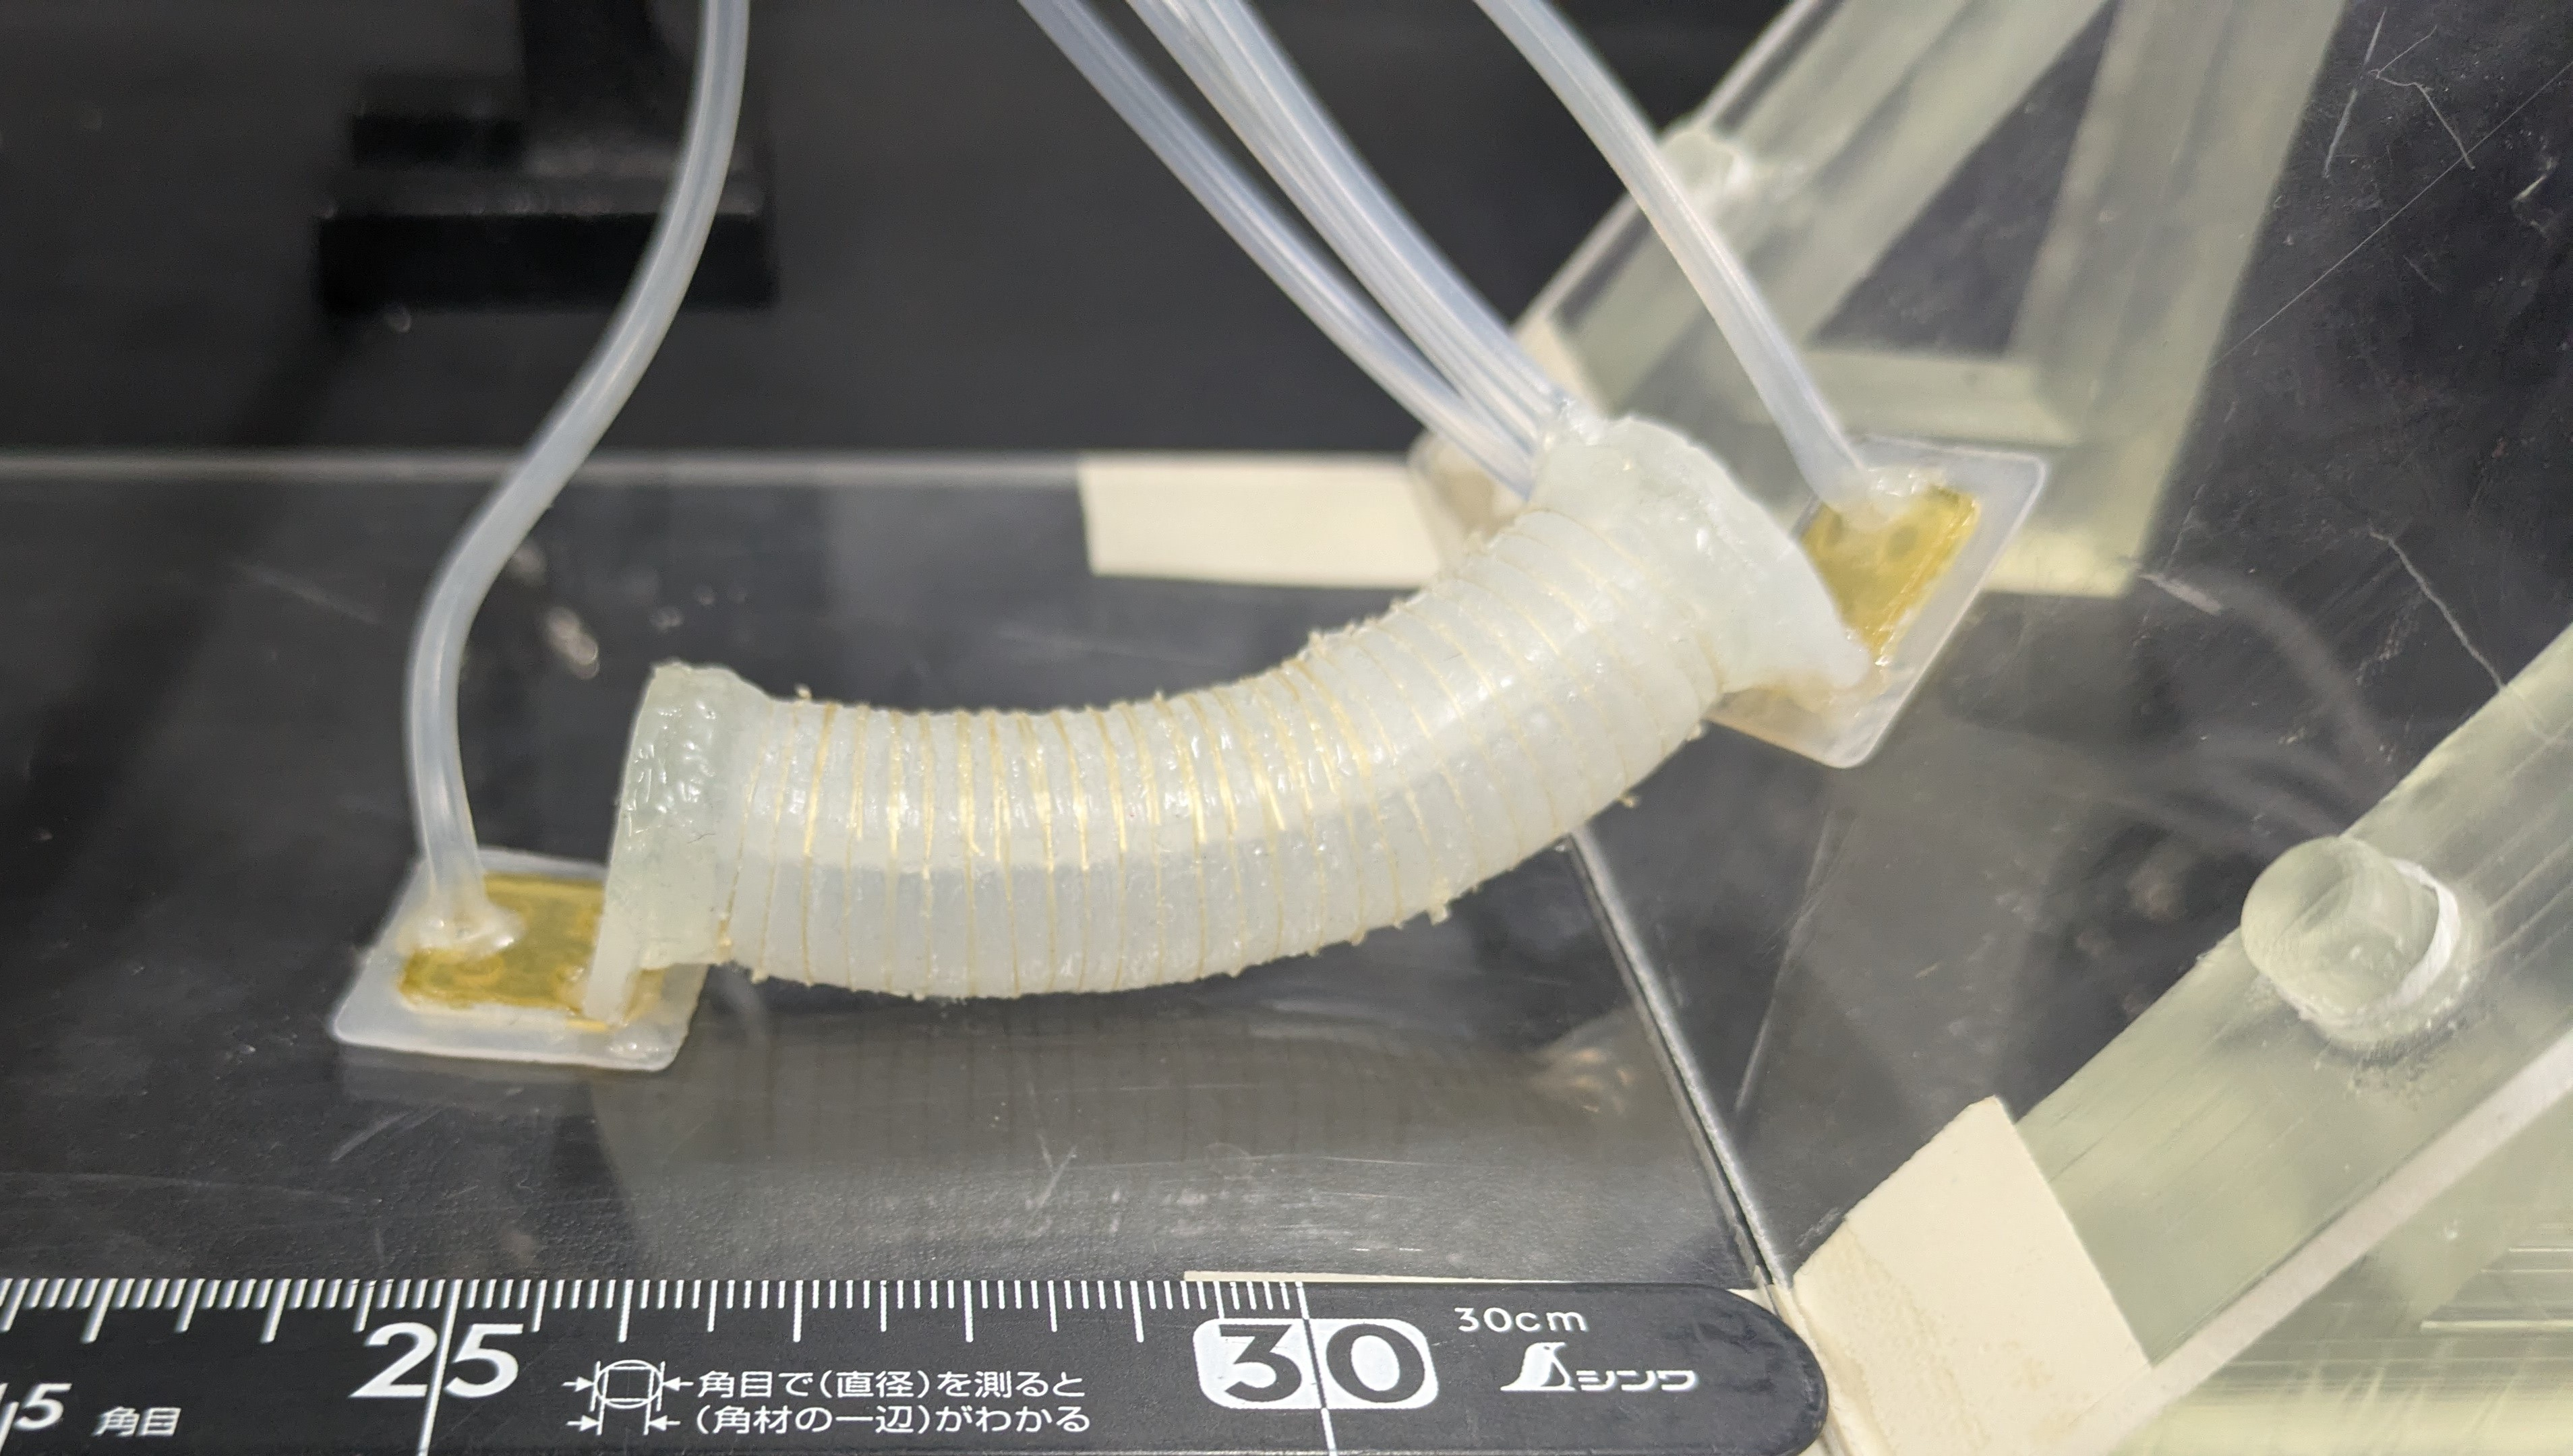
\includegraphics[width=0.185\textwidth]{figures/appendix_figures/7.jpg}\hfill
  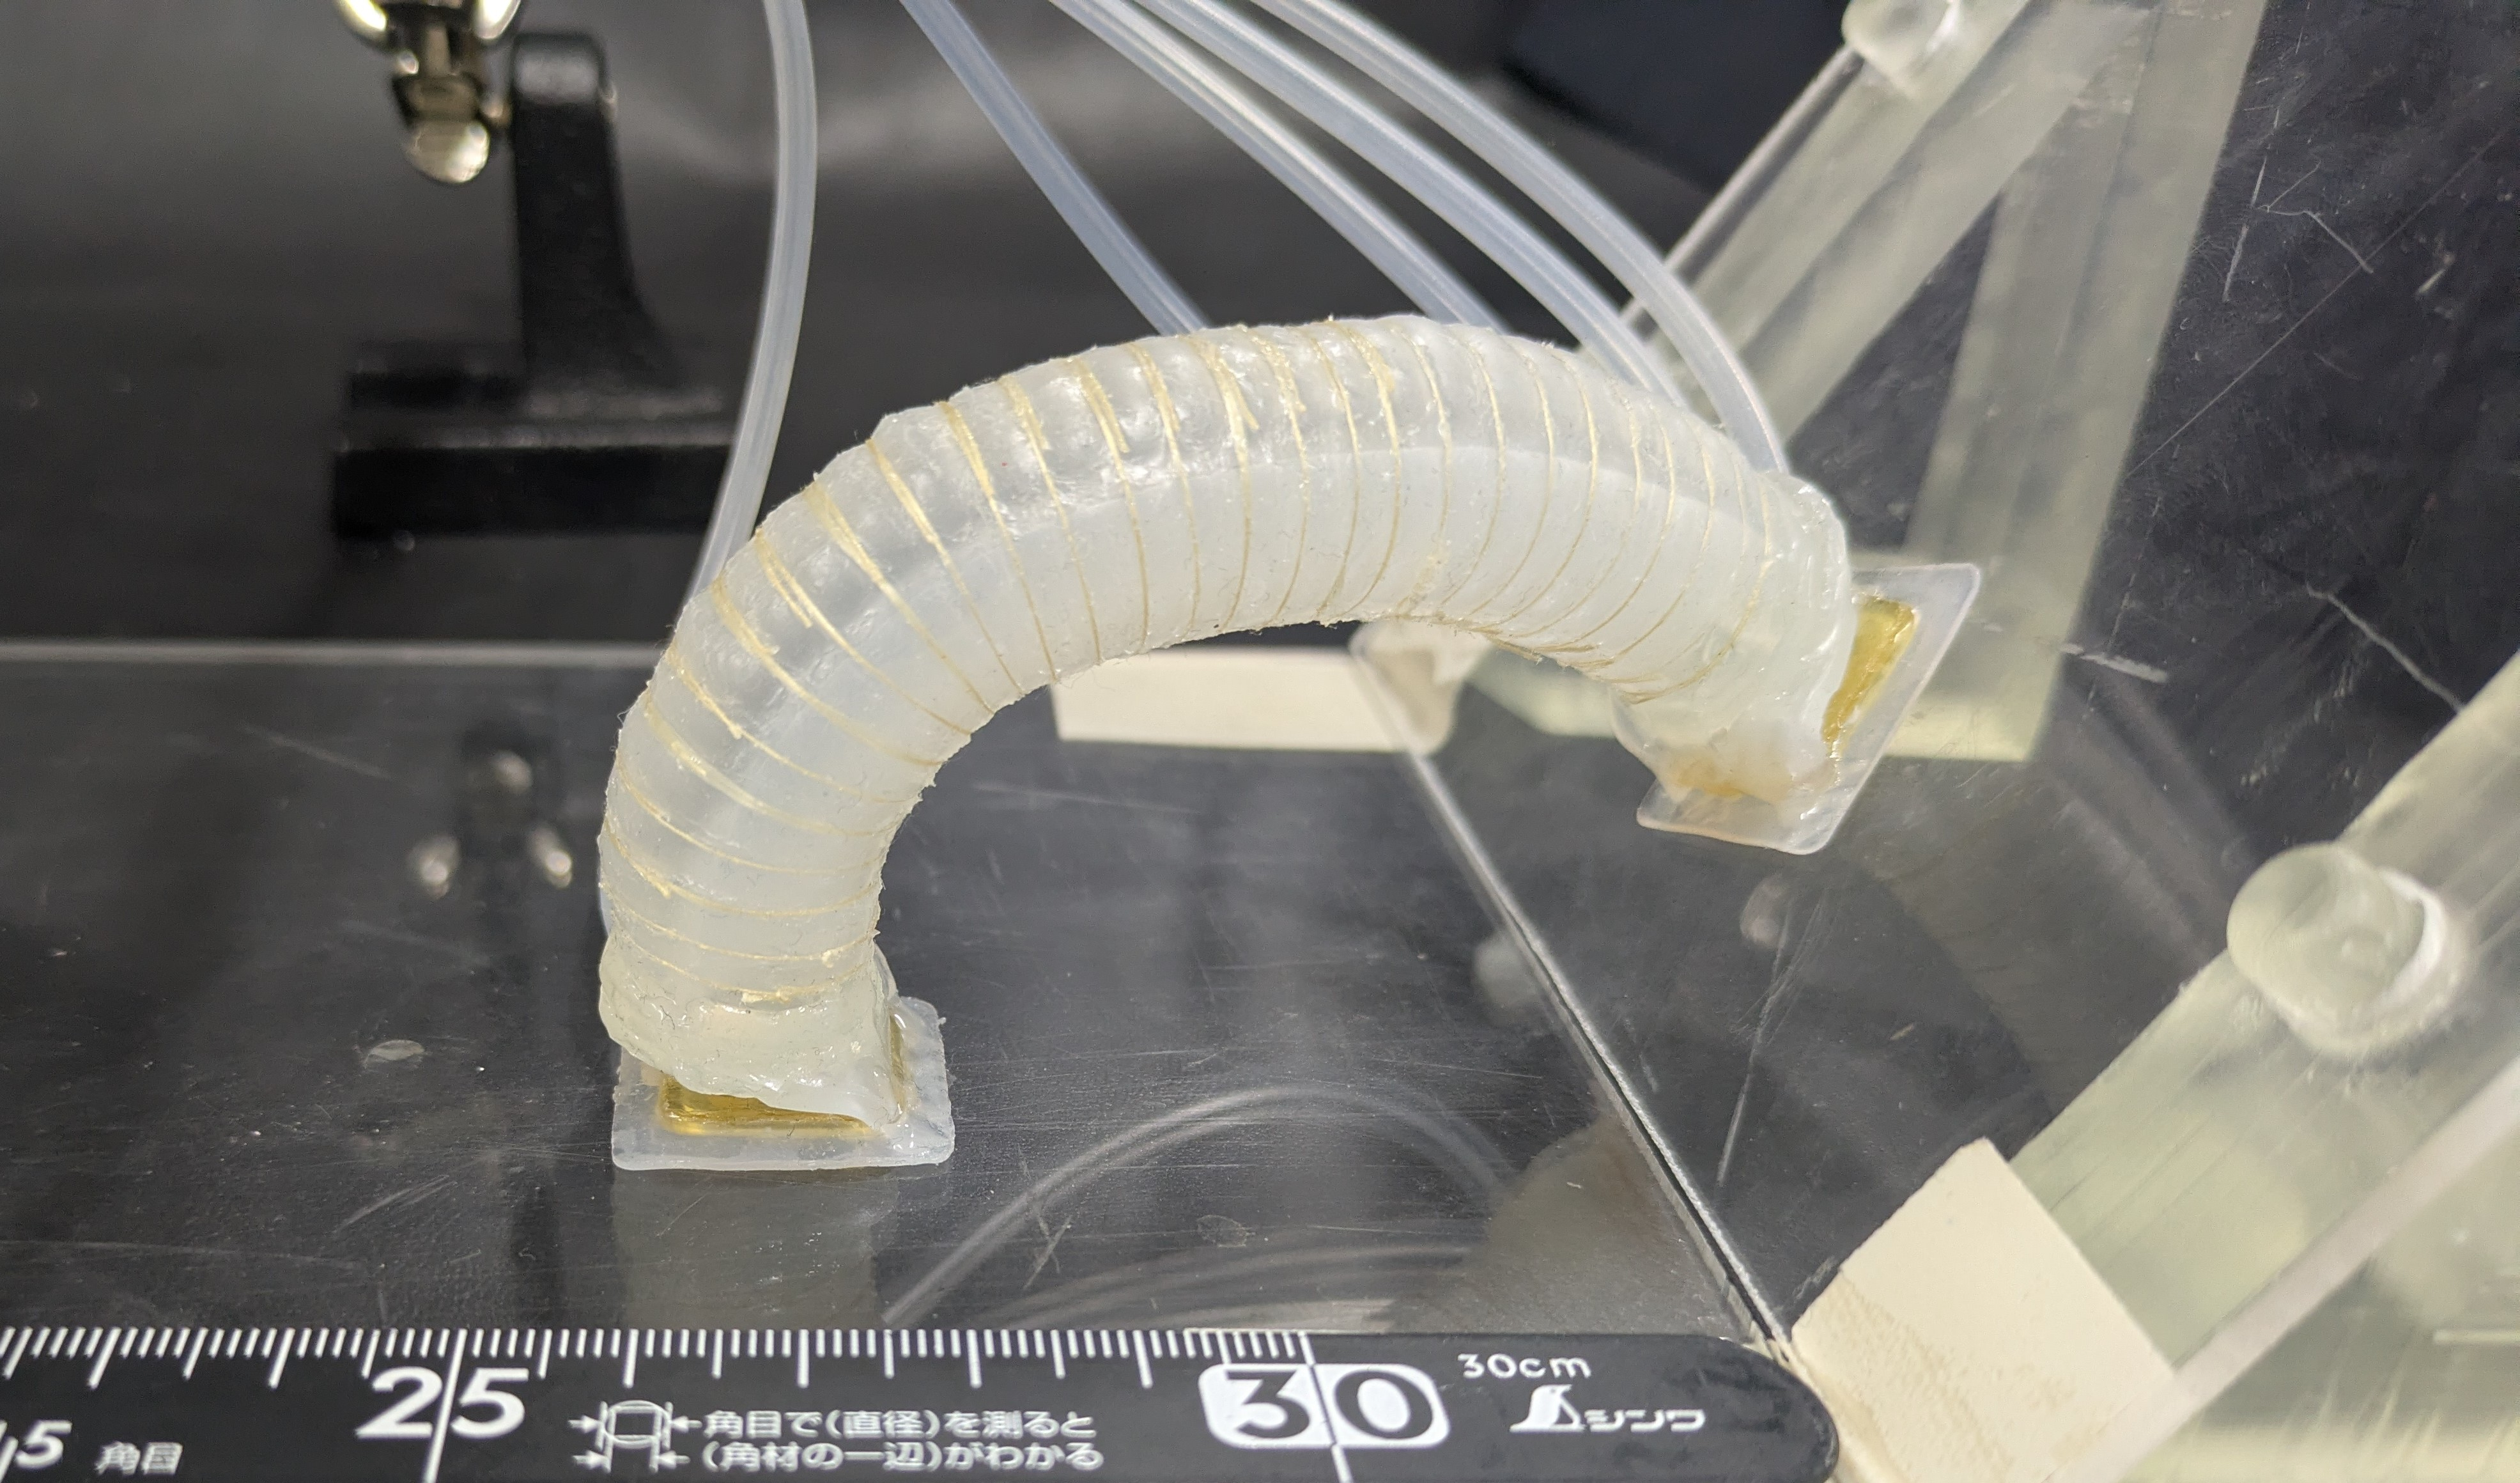
\includegraphics[width=0.185\textwidth]{figures/appendix_figures/8.jpg}\hfill
  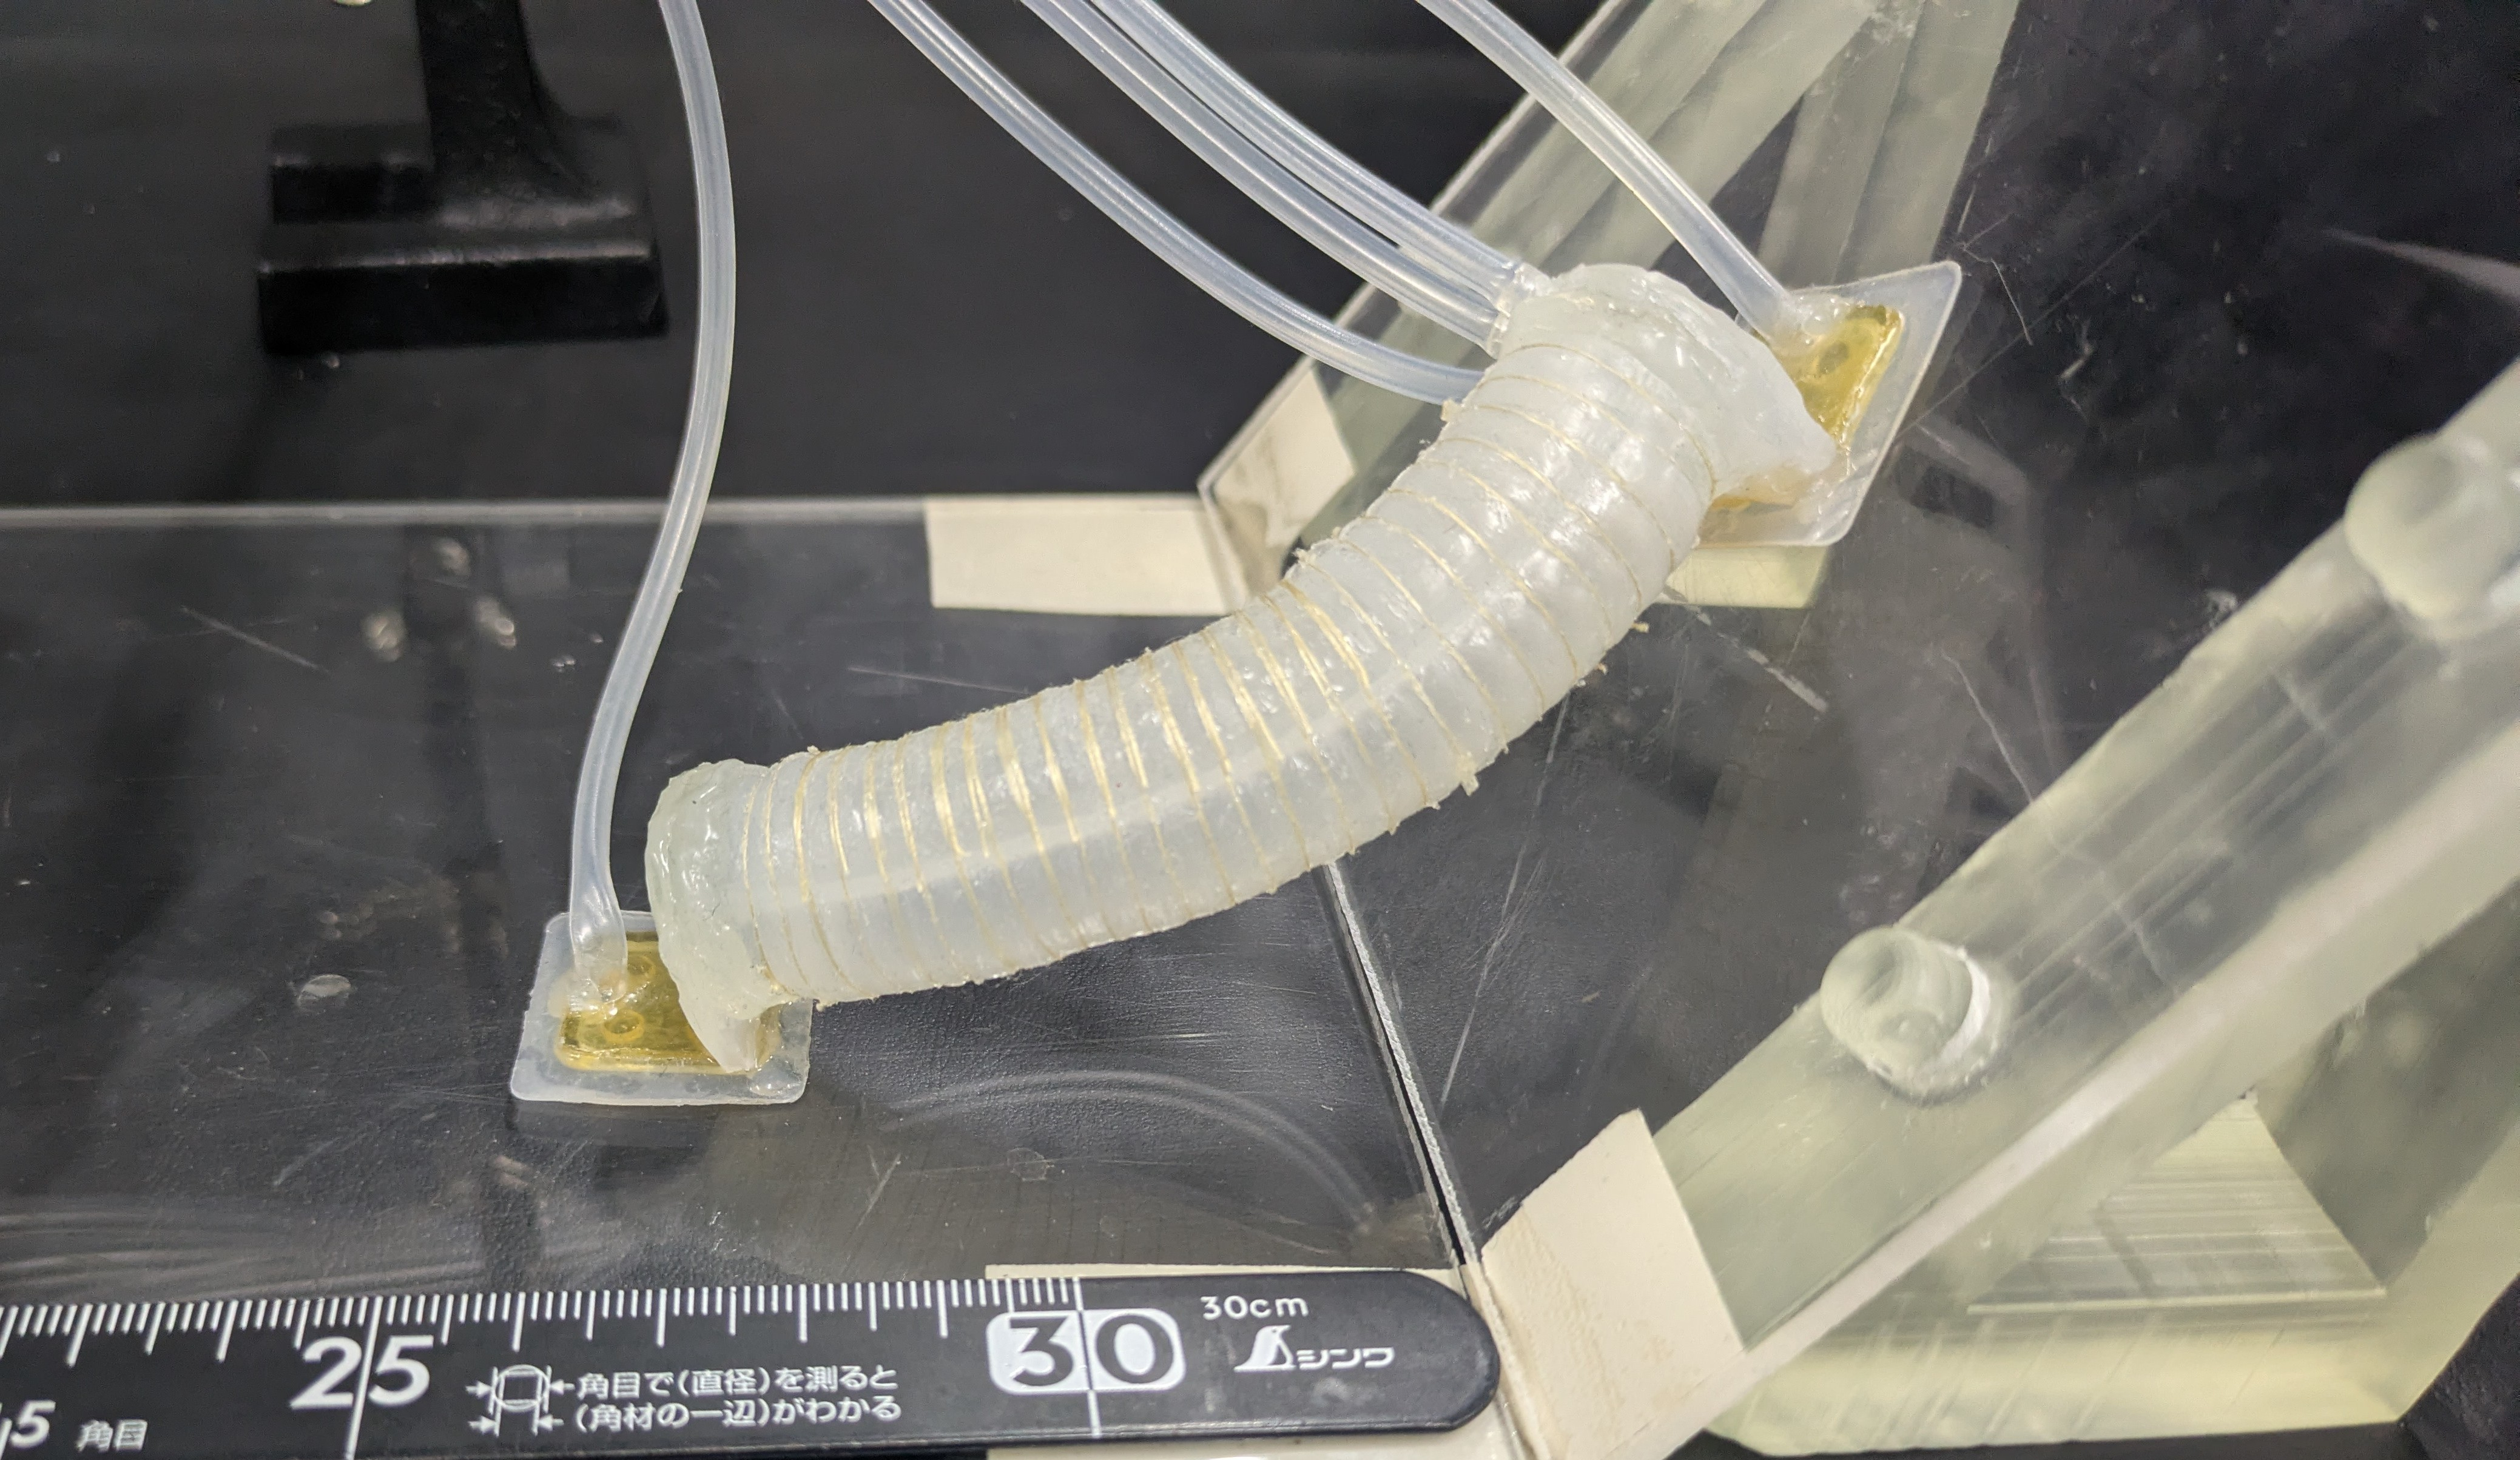
\includegraphics[width=0.185\textwidth]{figures/appendix_figures/9.jpg}\hfill
  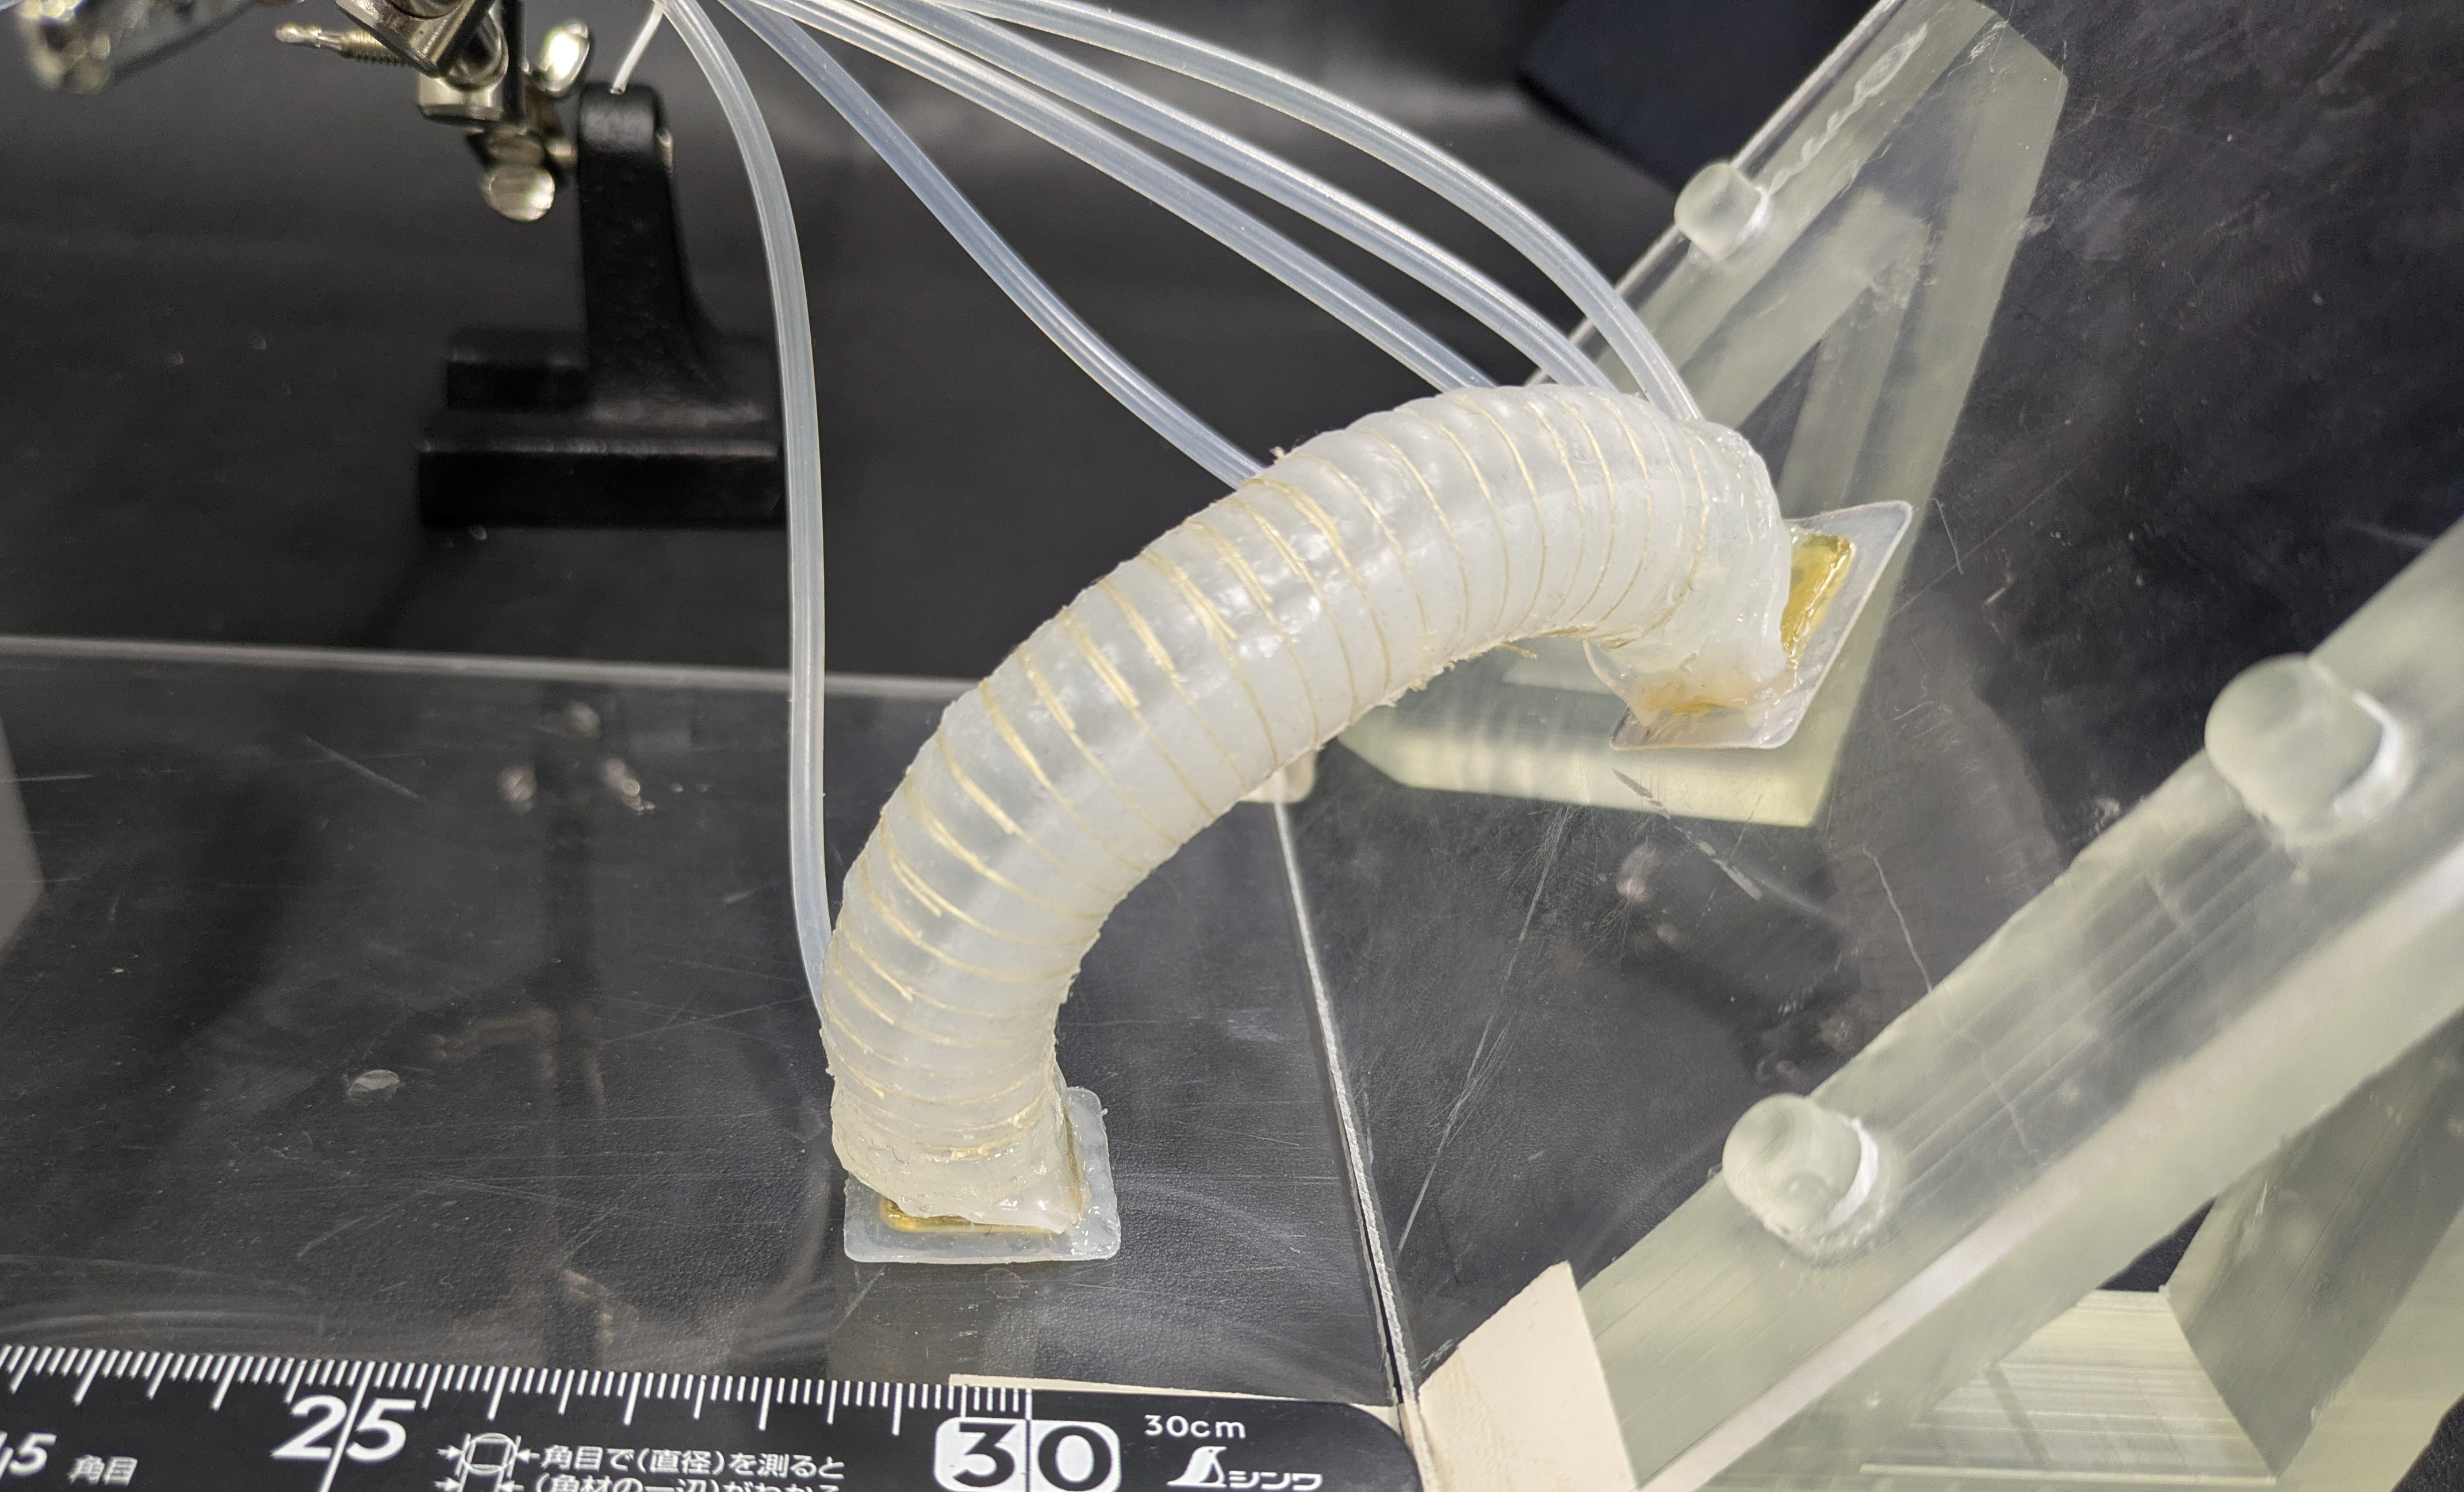
\includegraphics[width=0.185\textwidth]{figures/appendix_figures/10.jpg}
  \\[1.5mm]
  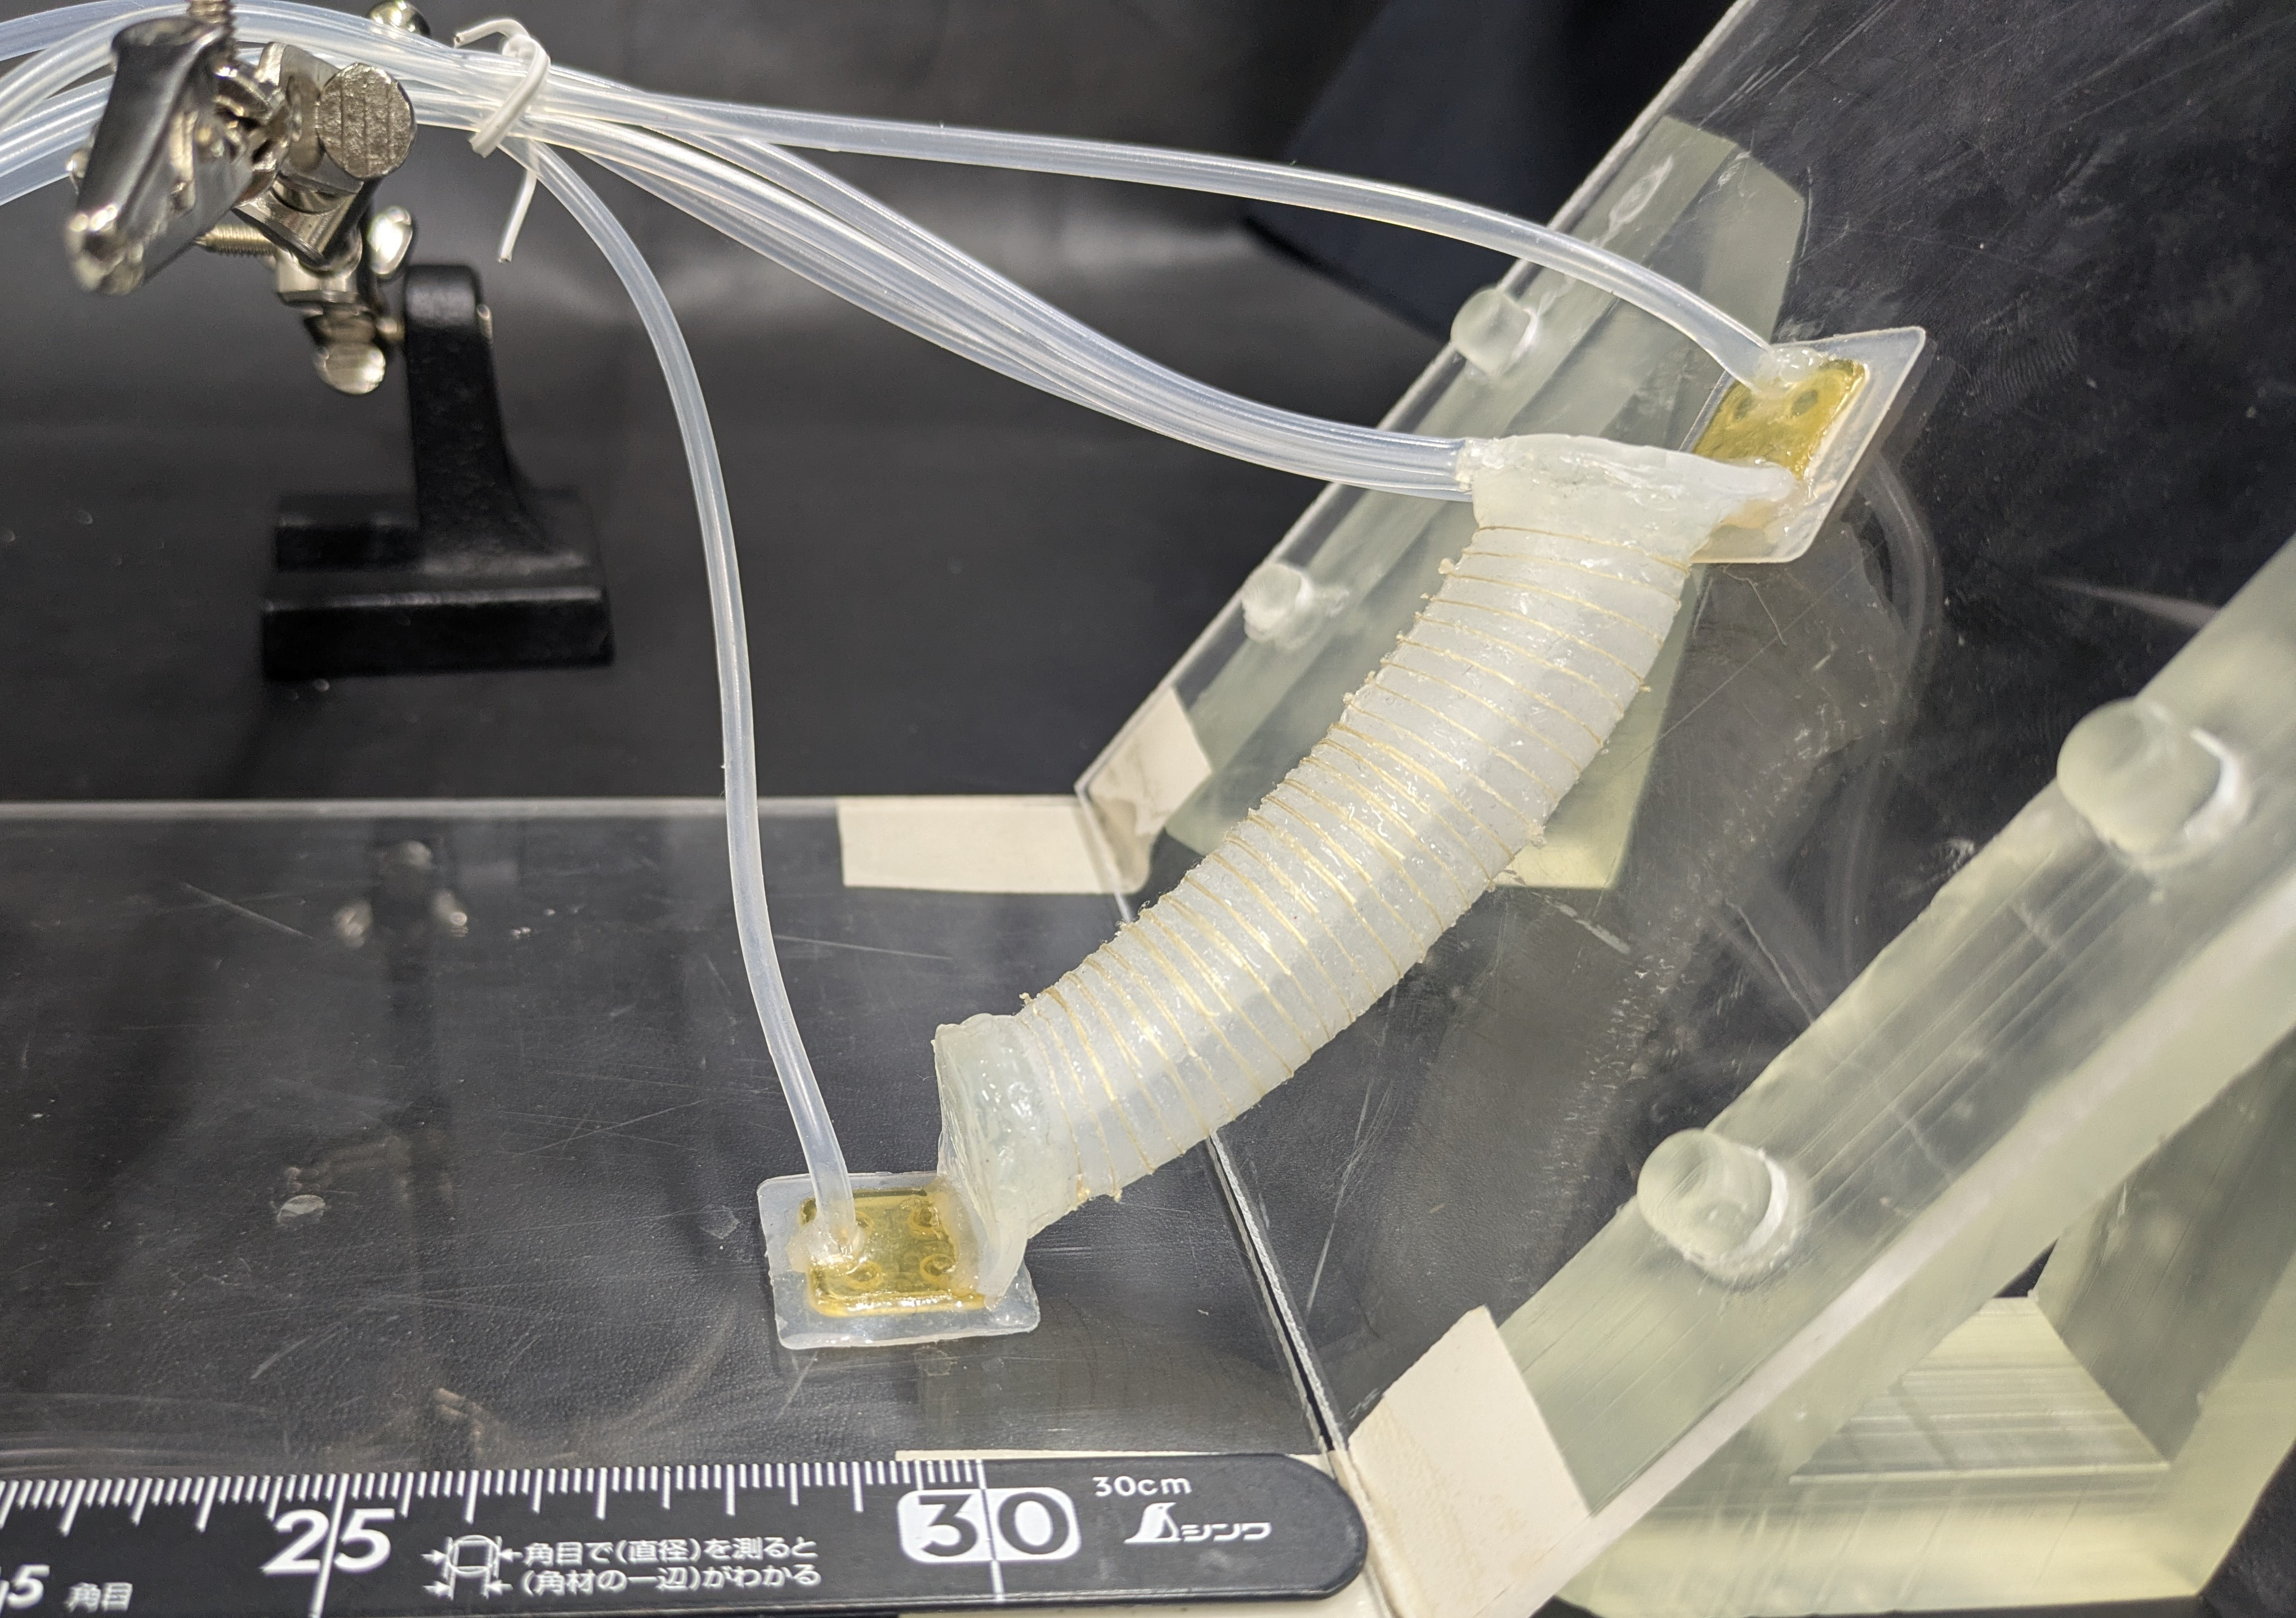
\includegraphics[width=0.185\textwidth]{figures/appendix_figures/11.jpg}\hfill
  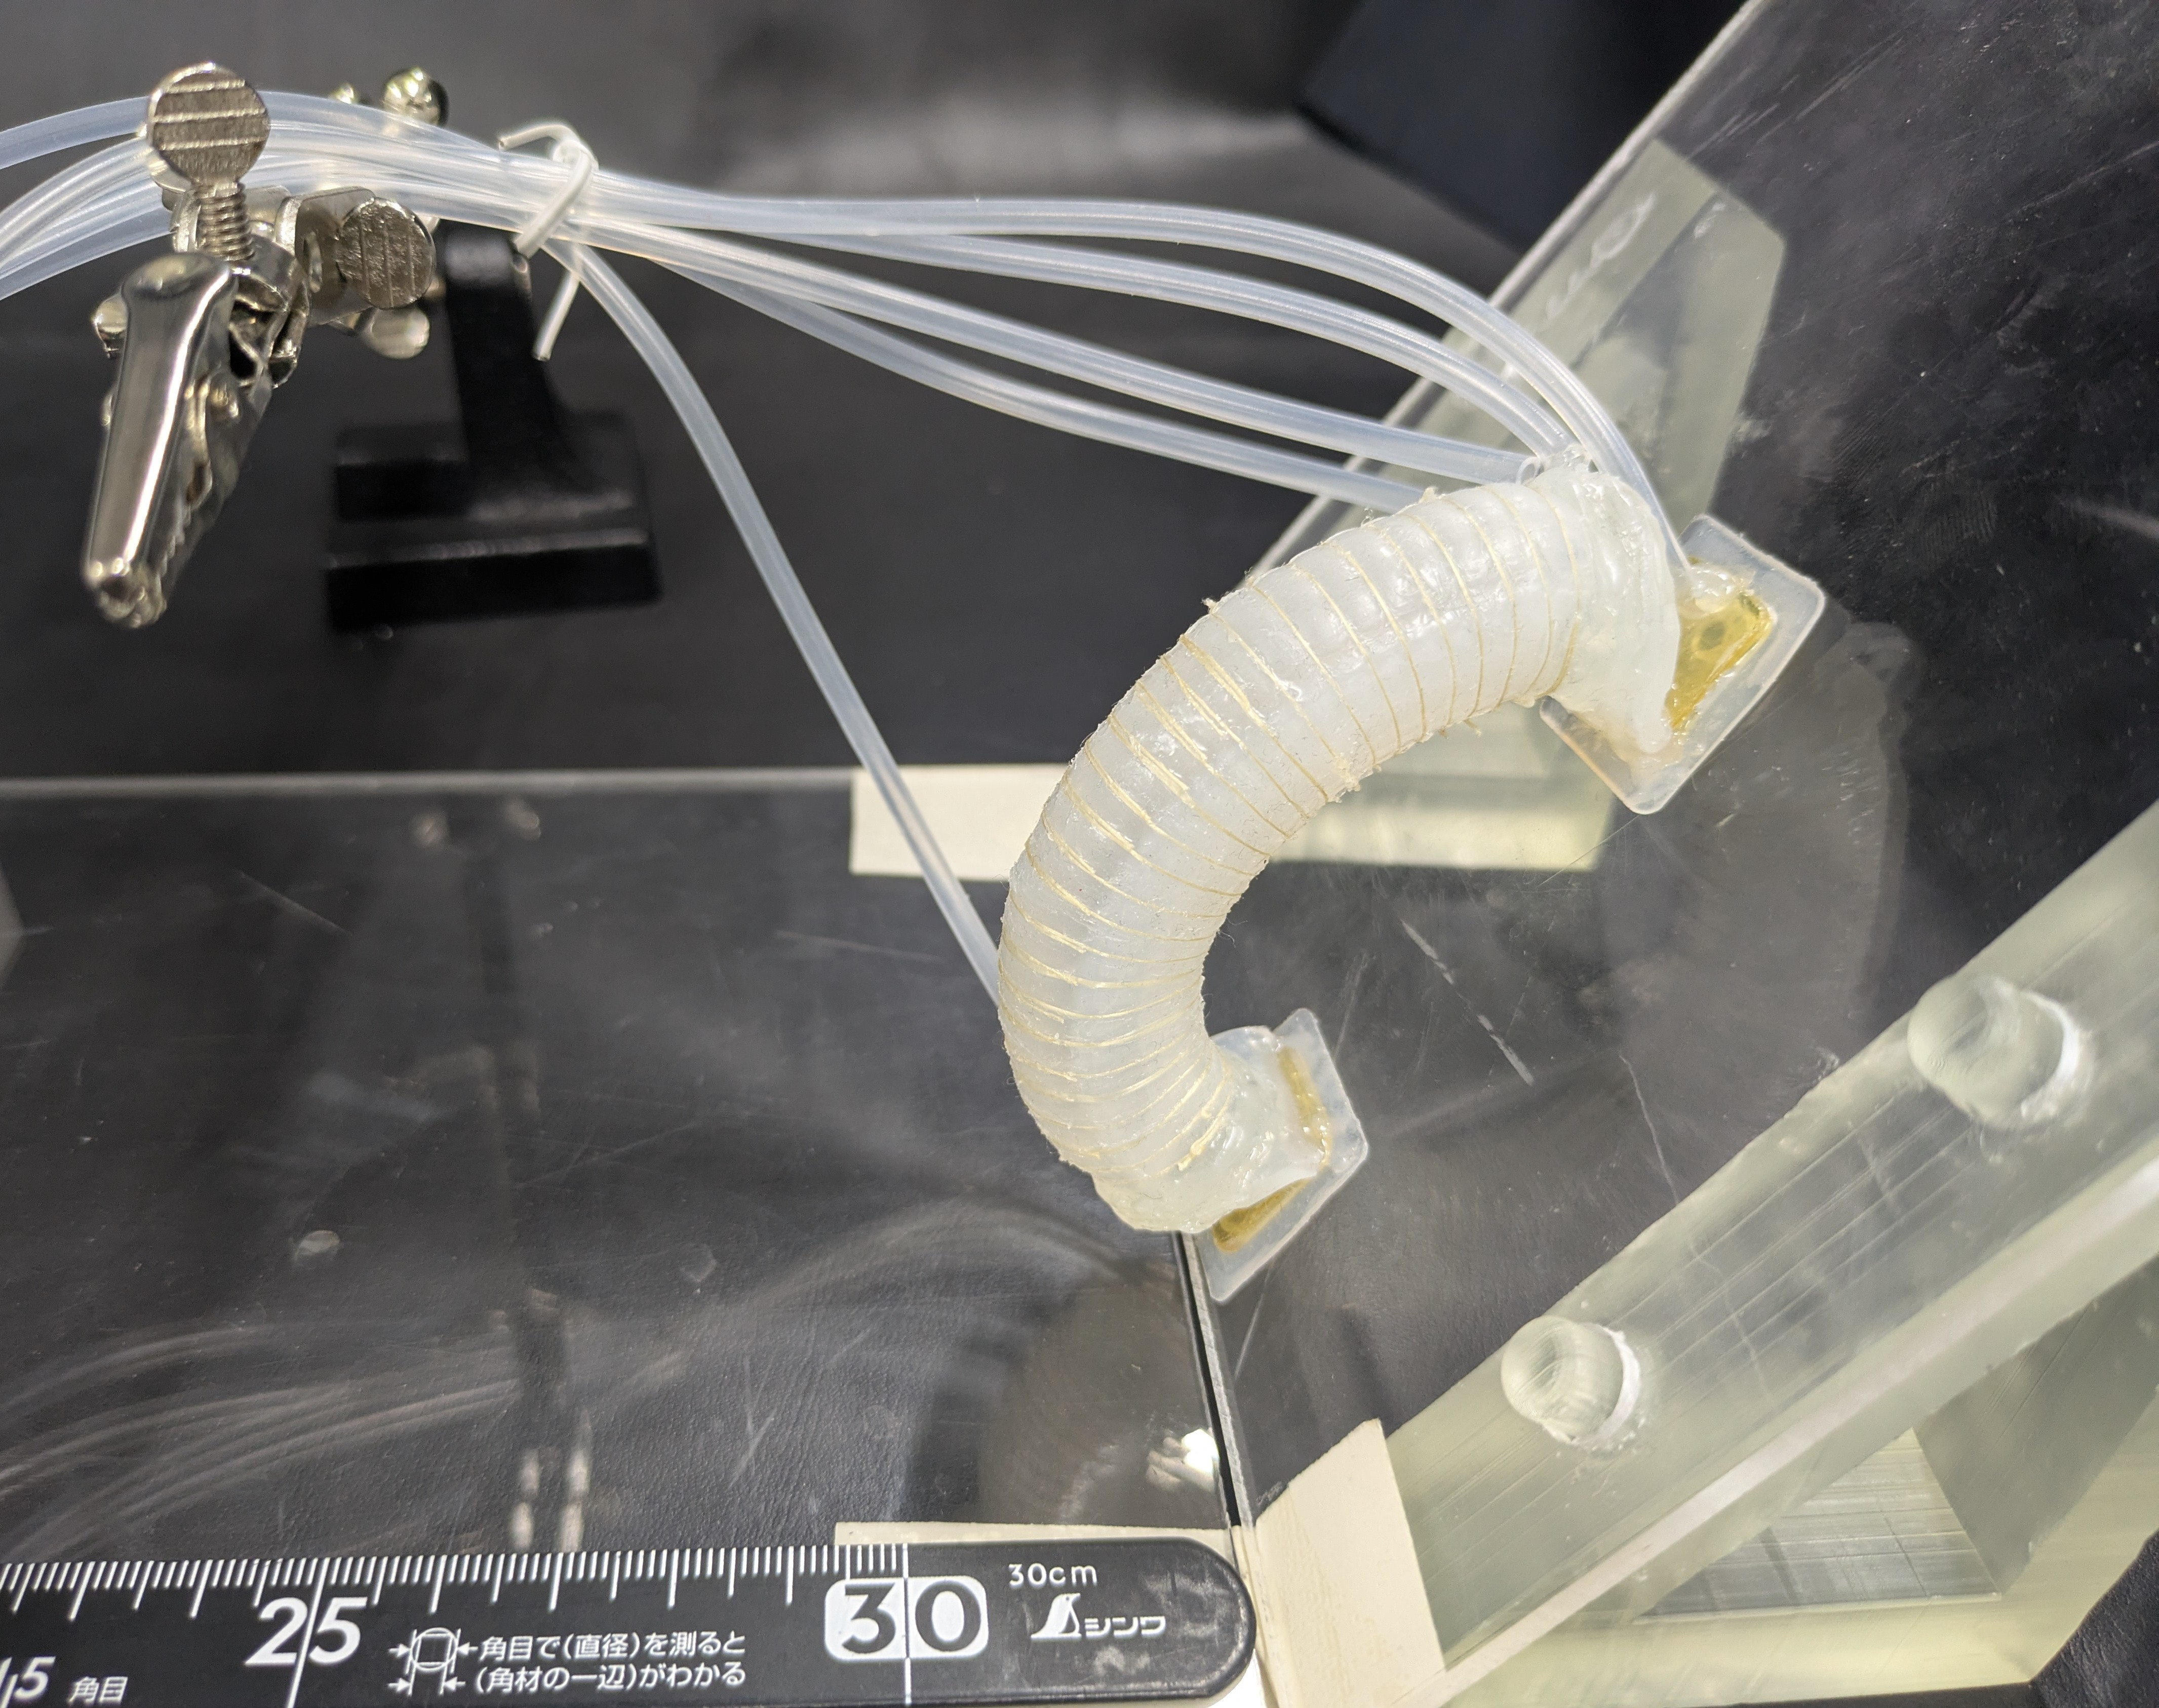
\includegraphics[width=0.185\textwidth]{figures/appendix_figures/12.jpg}\hfill
  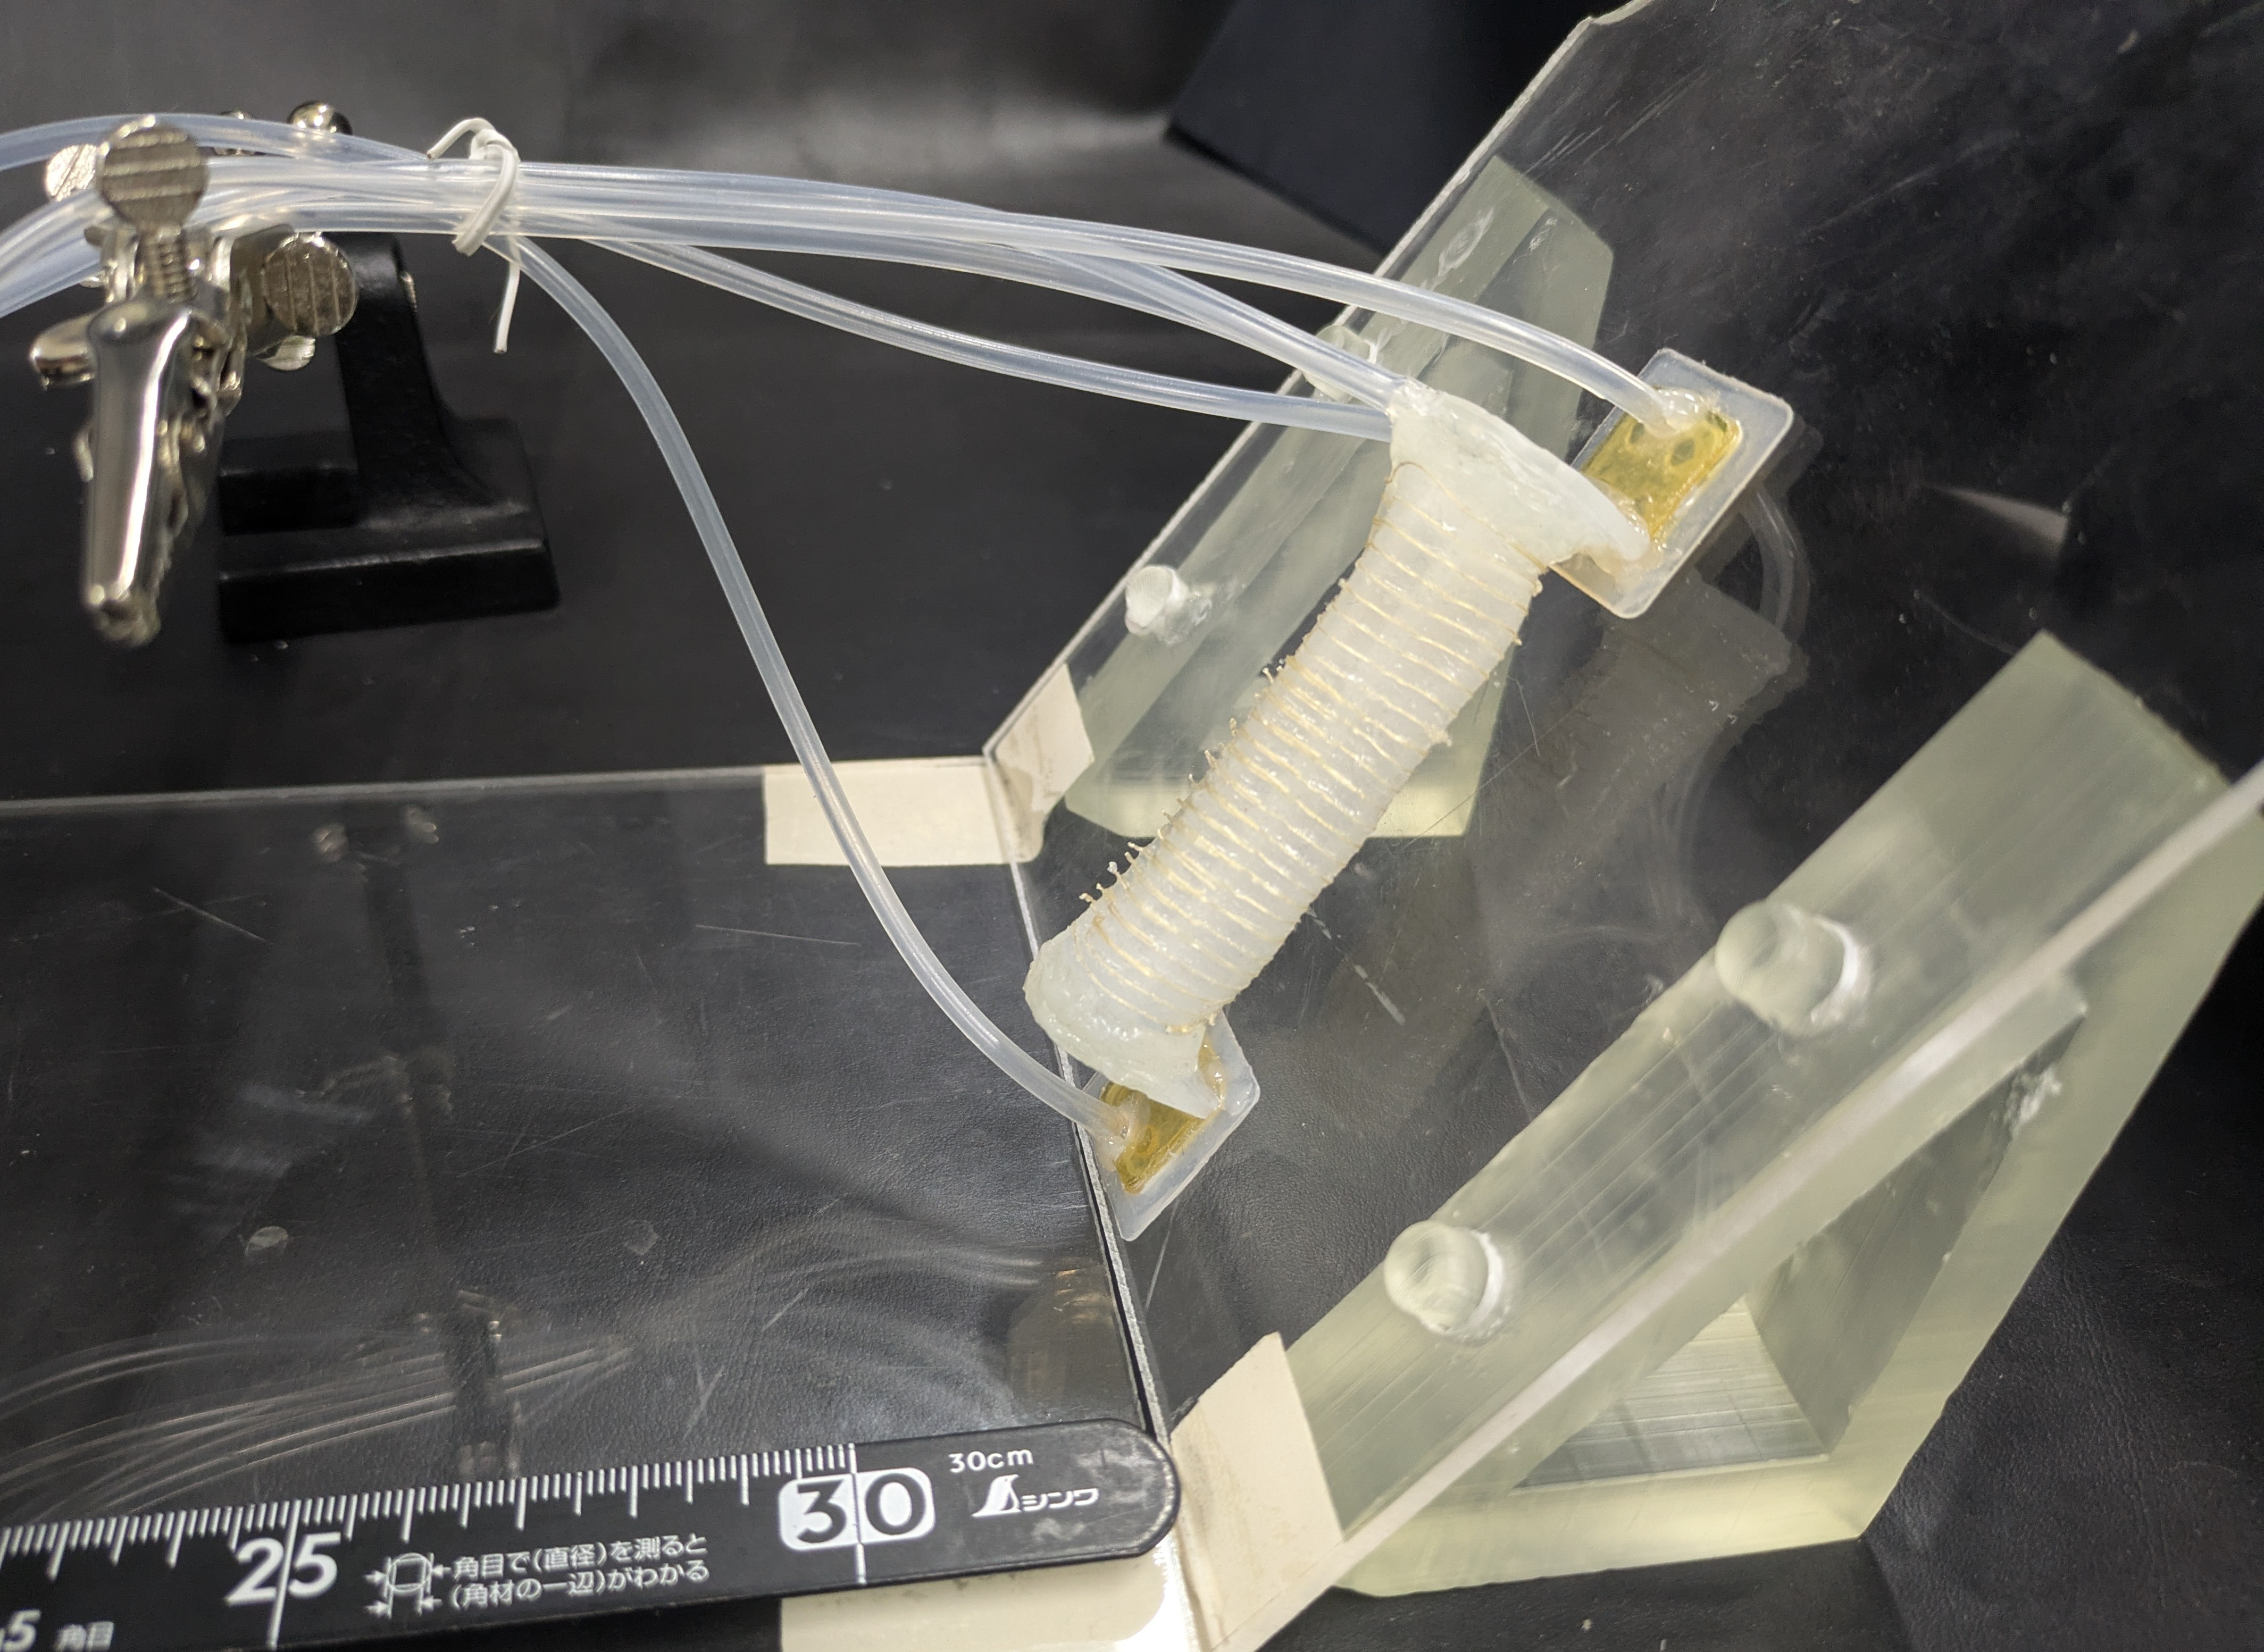
\includegraphics[width=0.185\textwidth]{figures/appendix_figures/13.jpg}\hfill
  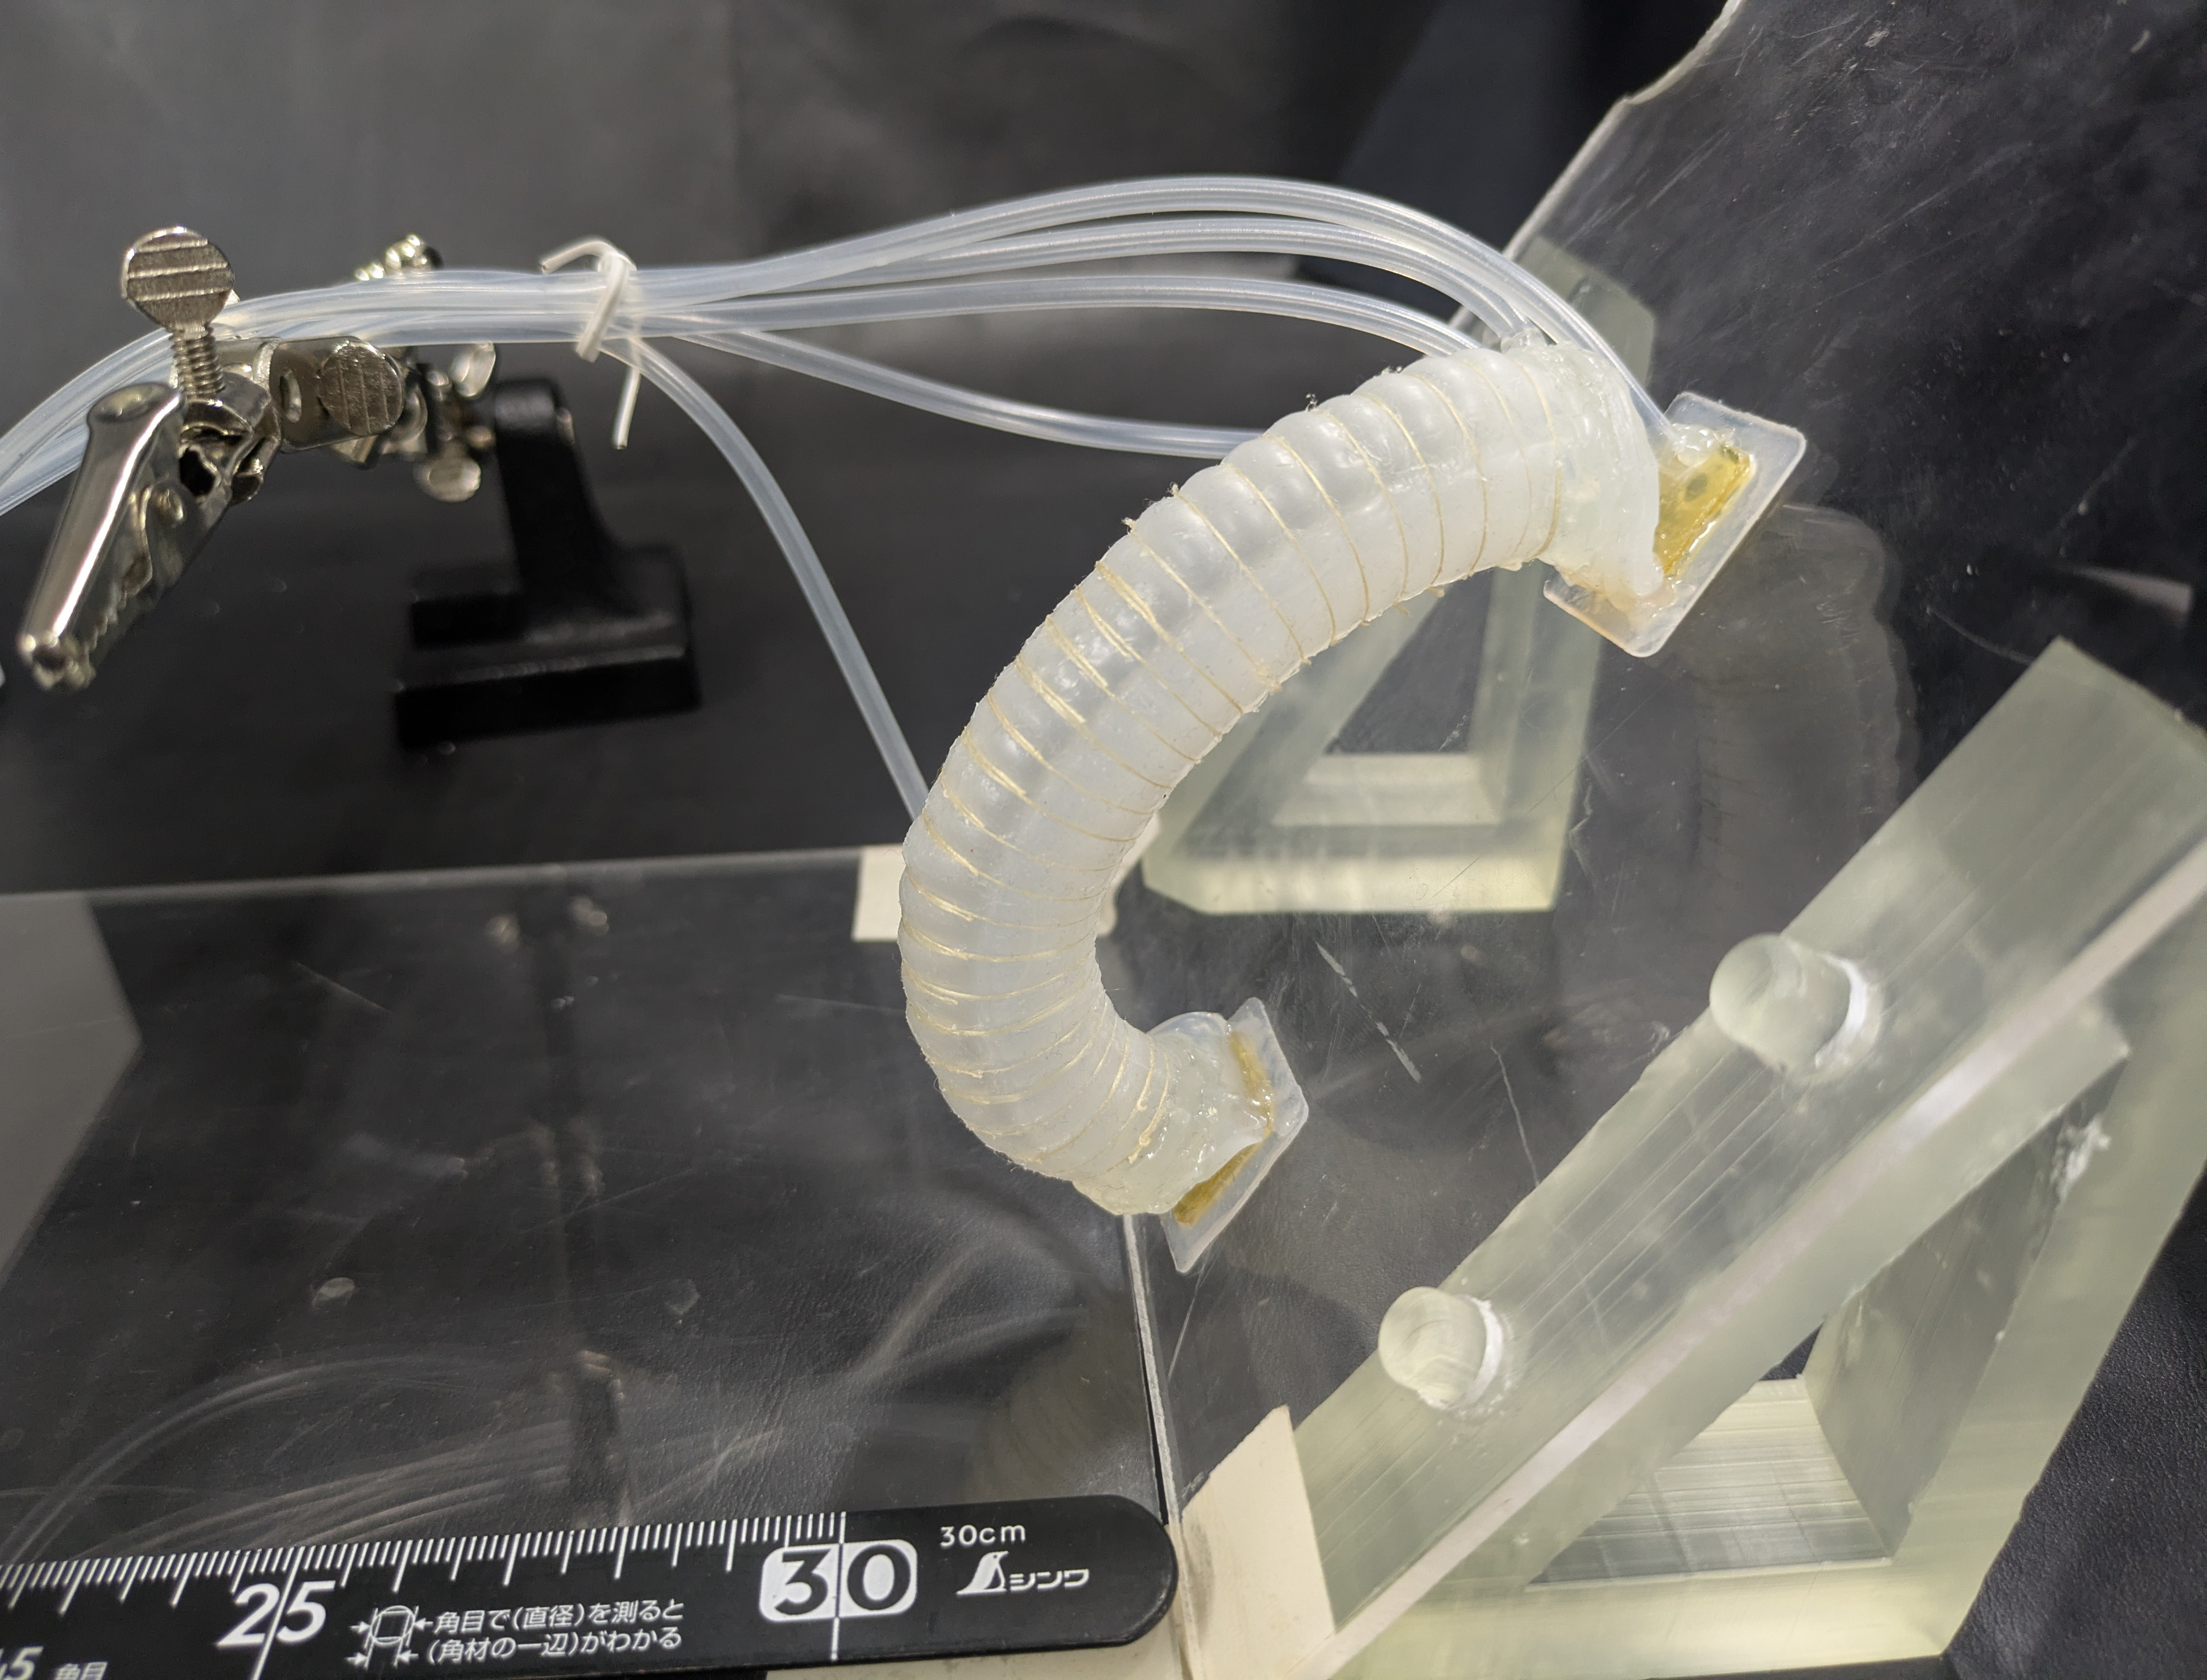
\includegraphics[width=0.185\textwidth]{figures/appendix_figures/14.jpg}\hfill
  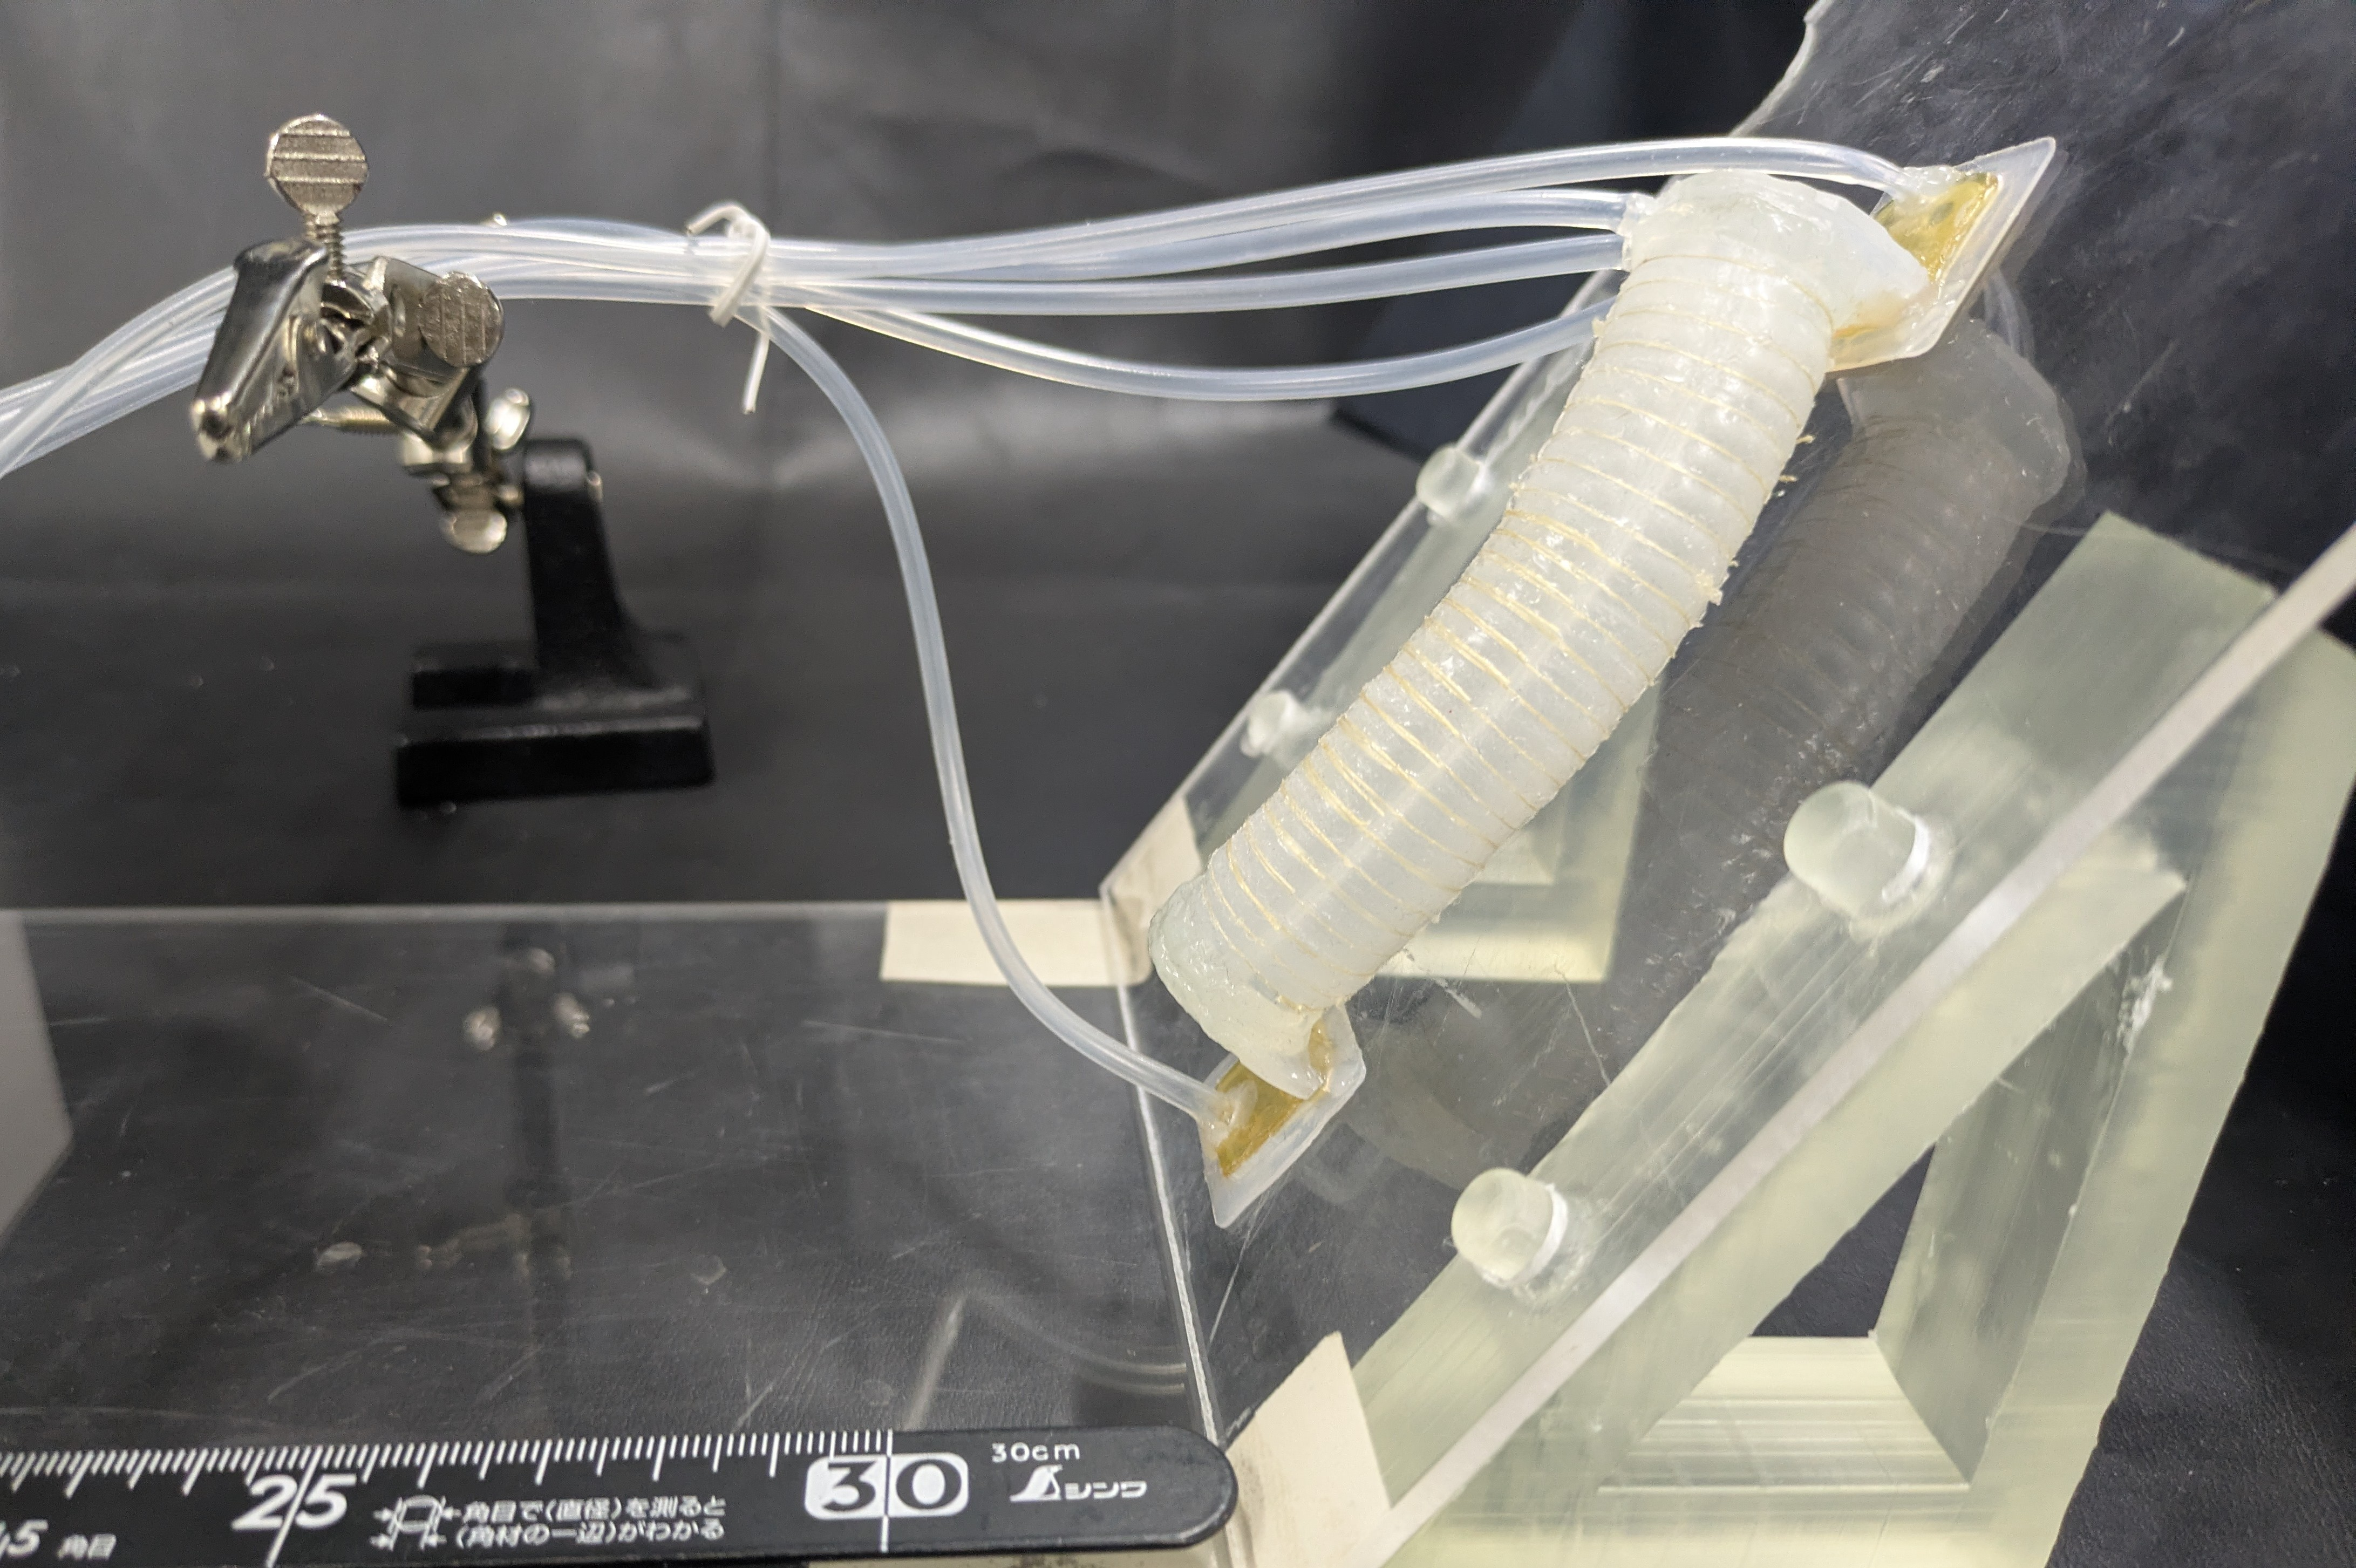
\includegraphics[width=0.185\textwidth]{figures/appendix_figures/15.jpg}
  \vspace*{-1mm}
  \caption{Complete 15-step floor-to-wall transition sequence of the soft
  inchworm robot on a $60^\circ$ incline (steps 1--15, left to right, top to
  bottom), corresponding to the summary in
  Fig.~\ref{fig:inchworm-transition}.}
  \label{fig:app-transition-sequence}
\end{figure*}
